\chapter{Differential networks reveal the dynamics of animal injury and disease co- occurrences}

\subsection{Introduction}
Rice (\textit{Oryza sativa}) is a major crop in South and Southeast Asian. The Food and Agriculture Organization of the United Nations (FAO) estimates that approximately 70 percent of total lowland rice area produces tow rice crops each year. The first crop is cultivated in the wet season, while another is in the dry season. The important role of seasonal cropping in the temporal dynamics of animal pests and diseases has been studied under farmers field survey in South and Southeast Asia by the use of multivariate techniques \citet{Savary_2000_Characterization, Willocquet_2008_Simulating}. These studies showed that injuries profiles (the combination of injuries) differ from season to season due to weather patterns, which in dry season, crop losses were lower than in the wet season because of lower incidence and severity of pests and diseases \citep{Litsinger_1991_Crop}. Additional a previous study based on surveys done in farmers’ rice fields in the region of lowland rice were shown that injury profiles were strongly associated with season.

In the previous chapter, the co-occurrence networks showed  co-occurrence networks, a methodological approach which has already proved fruitful in a variety of different applications.  Plant injuries caused by pests maybe affect yield production. Therefore, in this chapter, I attempted to characterize the patterns of rice injuries by studying the changes in the co-occurrence patterns of rice injuries (\textit{e.g} disease incidence, animal pest injury incidence) in different season and different yield levels.

Differential network analysis aims to compare the connectivity of two nodes at two different conditions. As demonstrated by several studies, differential networks can identify important nodes implicated in my fields, and also provide critical novel insights not obtainable using other approaches. In this work, I explore the the properties of network of a complex association of rice injuries at different yield levels. Elucidating the rice injuries association represents a key challenge, not only for achieving a deeper understanding of injury association (injury profiles) but also for identifying the unique association. Given that the injury association is governed by a complex network of injuries association, it seems natural to explore network properties which may help elucidate some of different association presenting in the different seasons.

In this chapter, I employ a differential network topology method to examine the co-occurrence relationships of rice injuries from survey data. I use graph theory methods to examine the topological feature dynamic of a co-occurrence network corresponding to different seasons, and production environments. The co-occurrence networks were built from differentially co-occurring injuries. I extract significantly differential co-occurring injuries from co-occurrence networks, which represent different seasons, to identify which injuries that may be involved specifically curtain season. I postulate that these selected injuries may contribute to the difference in the co-occurrence patterns in different season. Furthermore, I identified the injuries associated with yield from networks at different yield levels. Finally, I suggest key injuries that may contribute to yield reduction under a curtain production environment. The goal is to leverage insights to better understand the rice injury co-occurrence that may contribute to pest management development.

\newpage
\subsection{Materials and Methods}

\textbf{Differential co-occurrence network construction}

The survey data were pre-processed by using methods described in the previous chapter. Subsequently, I applied the method proposed by \citet{Fukushima_2013_Diffcorr} to identify differentially co-occurrence links. The difference of co-occurrence of injury $x$ and $y$ between two conditions ($A$ and $B$) was quantified by Fisher's $z$-test.
 
For the pair of $x$ injury and $y$ injury, I denoted the correlation coefficient based on Spearman's correlation coefficient by $r_{xy}^A$ and $r_{xy}^A$ in networks of condition $A$ and condition $B$, respectively. To test whether the 2 correlation coefficients were significantly different, correlation coefficients for each of the 2 conditions, $r_{xy}^A$ and $r_{xy}^B$, were transformed into $Z_{xy}^A$ and $Z_{xy}^B$, respectively.


The Fisher's transformation of coefficient $r_{xy}^A$ is defined by
\begin{equation}
\label{eq:zvalue}
Z_{xy} = \frac{1}{2} \log\left[{\frac{1 + r_{xy}}{1 - r_{xy}}}\right]
\end{equation}

Next, The $p$-value of the difference in $Z_{xy}$ values was calculated using the standard normal distribution.

\begin{equation}
\label{eq:pofz}
p(Z\geq \left | \frac{Z_{xy}^A - Z_{xy}^B}{\sqrt{\frac{1}{N_{A}-3}+ \frac{1}{N_{A}-3}}} \right |
\end{equation}

Next, The $p$-value of the difference in Z values was calculated using the standard normal distribution

$N_{A}$ and $N_{A}$ represent the sample size for each of condition. The $Z$ has an approximately Gaussian distribution under null hypotheses that the population correlations are equal. The pairwise correlation significants are considered at $p$-value < 0.05.


\textbf{Differential co-occurrence network in different seasons}

Consider any two injuries $x$ and $y$ in the survey data, let $r_{xy}^D$ and $r_{xy}^W$ be the Spearman’s correlation coefficient calculated separately over the samples in dry and wet, respectively. I constructed differential co-occurrence networks that are specified by adjacency matrix $A^{diff}$ = $(A_{xy}^{diff})$ where the entry $A_{xy}^{diff}$ quantified by following:   


\begin{equation}
A_{xy}^{diff} = \left\{\begin{matrix}
 1 & \text{when } r_{xy}^D > r_{xy}^W \text{ at } P_{z_{xy}} \text{-value}  < 0.05  \\ 
 0 & \text{when } P_{z_{xy}}  \text{-value}  > 0.05                              \\ -1 & \text{when } r_{xy}^W > r_{xy}^D \text{ at } P_{z_{xy}} \text{-value}  < 0.05 \end{matrix}\right.\end{equation}


For this differential co-occurrence network,$A_{xy}^{diff}$ equals 1 depending on whether any injury pairs show significantly higher correlation coefficient of co-occurrence  in dry season than wet season, but -1 is vice versa, and if it equal 0, meaning that co-occurrence level of injury pairs were not different in dry and wet season. \ref{fig:pipeline3} illustrated the differential co-occurrence network at different seasons.

\begin{figure}[h]
\centering
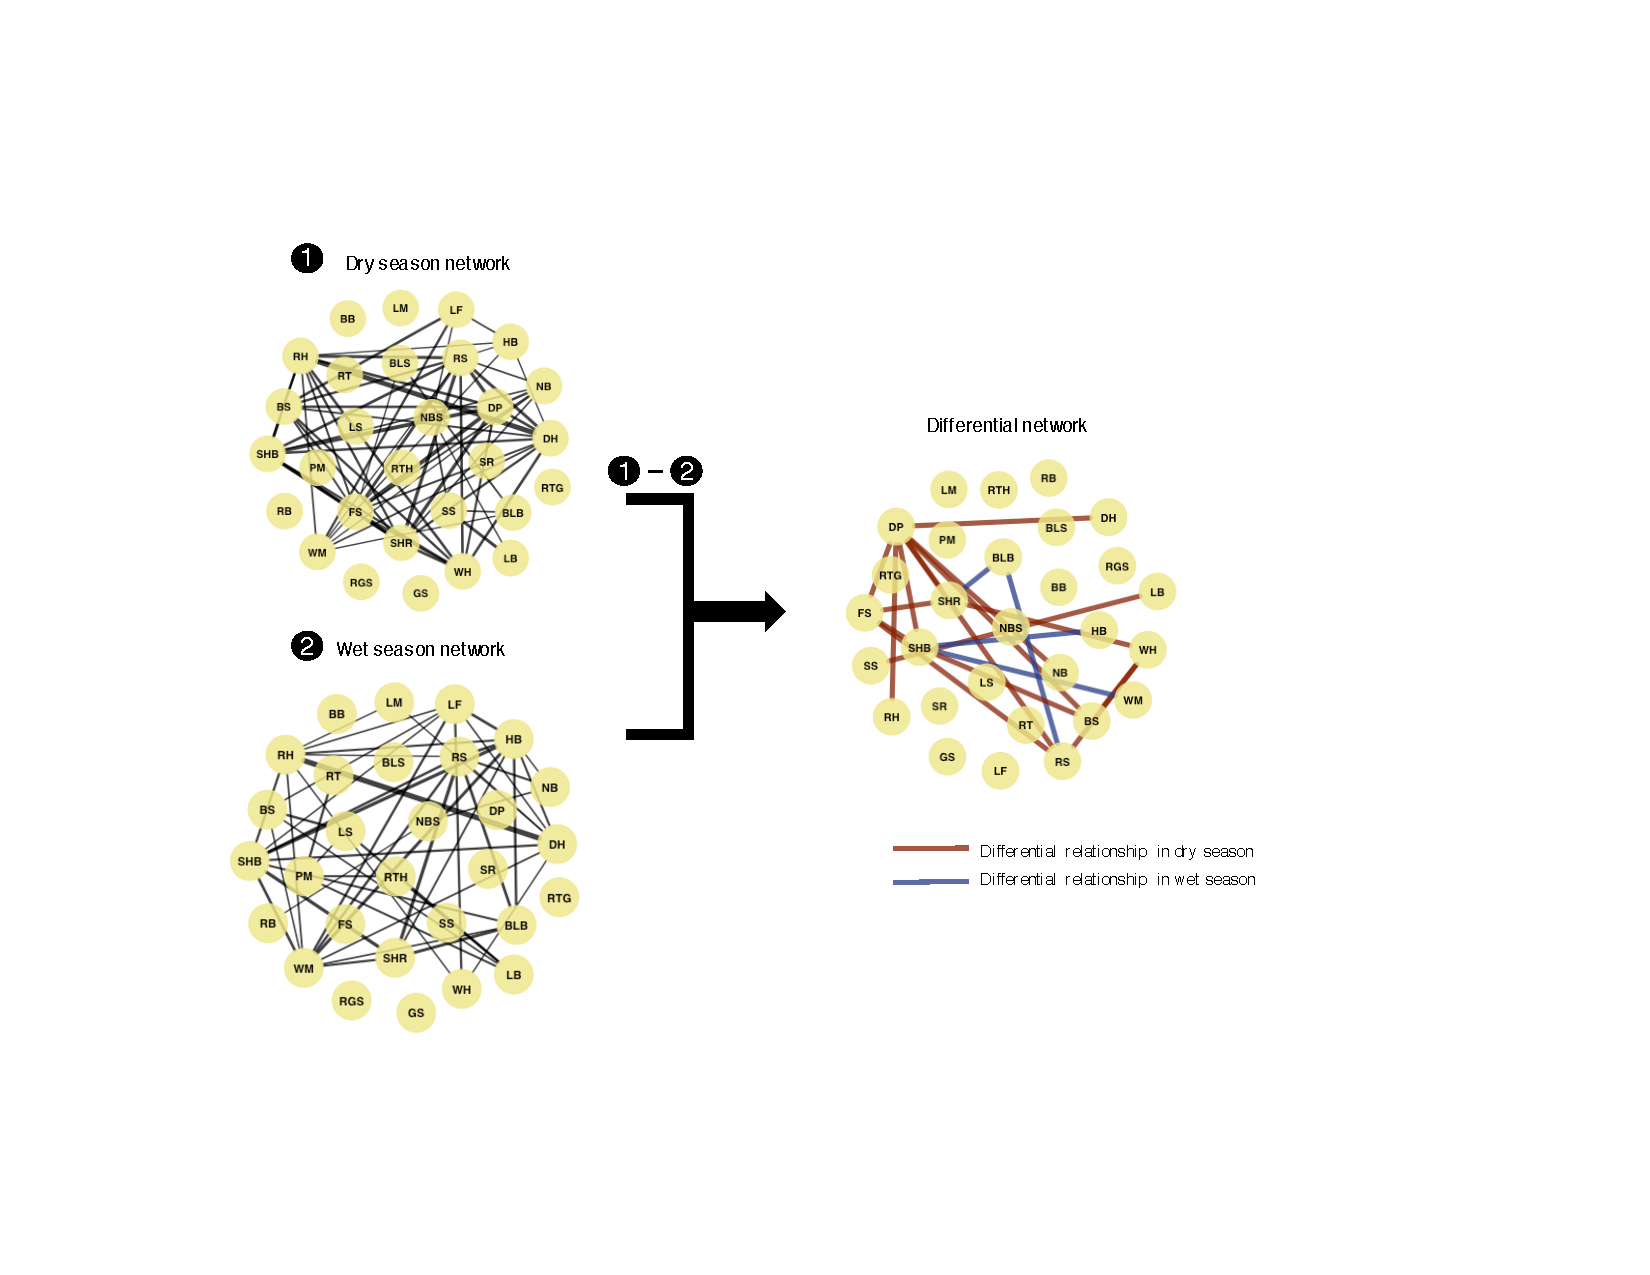
\includegraphics[width = 1\textwidth]{figures/pipeline3.pdf}
\caption[Differential analysis of crop health survey data in season]{Schematic showing differential analysis in seasons. Co-occurrence networks are measured in each of two seasons (left) resulting in interactions (black). Dry season is subtracted from wet season to create a differential co-occurrence network (right), in which the significant differential interactions are those that positive (red) or negative (blue) in score after the shift in conditions, which means differential in dry, and wet season, respectively.}
\label{fig:pipeline3}
\end{figure} 

\textbf{Difference of co-occurrence network of rice injuries at different yield levels}

Consider any two injuries $x$ and $y$ in the survey data, let $r_{xy}^L$ and $r_{xy}^H$ be the Spearman’s correlation coefficient calculated separately over the samples in $L$ and $H$ yield level, respectively. I constructed differential co-occurrence networks that are specified by adjacency matrix $A^{diff}$ = $(A_{xy}^{diff})$ where the entry $A_{xy}^{diff}$ quantified by following:   

\begin{equation}
A_{xy}^{diff} = \left\{\begin{matrix} 1 & \text{when } r_{xy}^L > r_{xy}^H \text{ at } P_{z_{xy}} \text{-value} < 0.05  \\  0 & \text{otherwise}                             
\end{matrix}\right.
\end{equation}

For  this differential co-occurrence network,$A_{xy}^{diff}$ equals 1 depending on whether any injury pairs show significantly higher co-occurrence level in low yield level than high yield state, and if it equal 0, meaning that co-occurrence level of injury pairs were not or lower different in low yield level state. \ref{fig:pipeline4} illustrated the differential co-occurrence network at different seasons.

\begin{figure}[h]
\centering
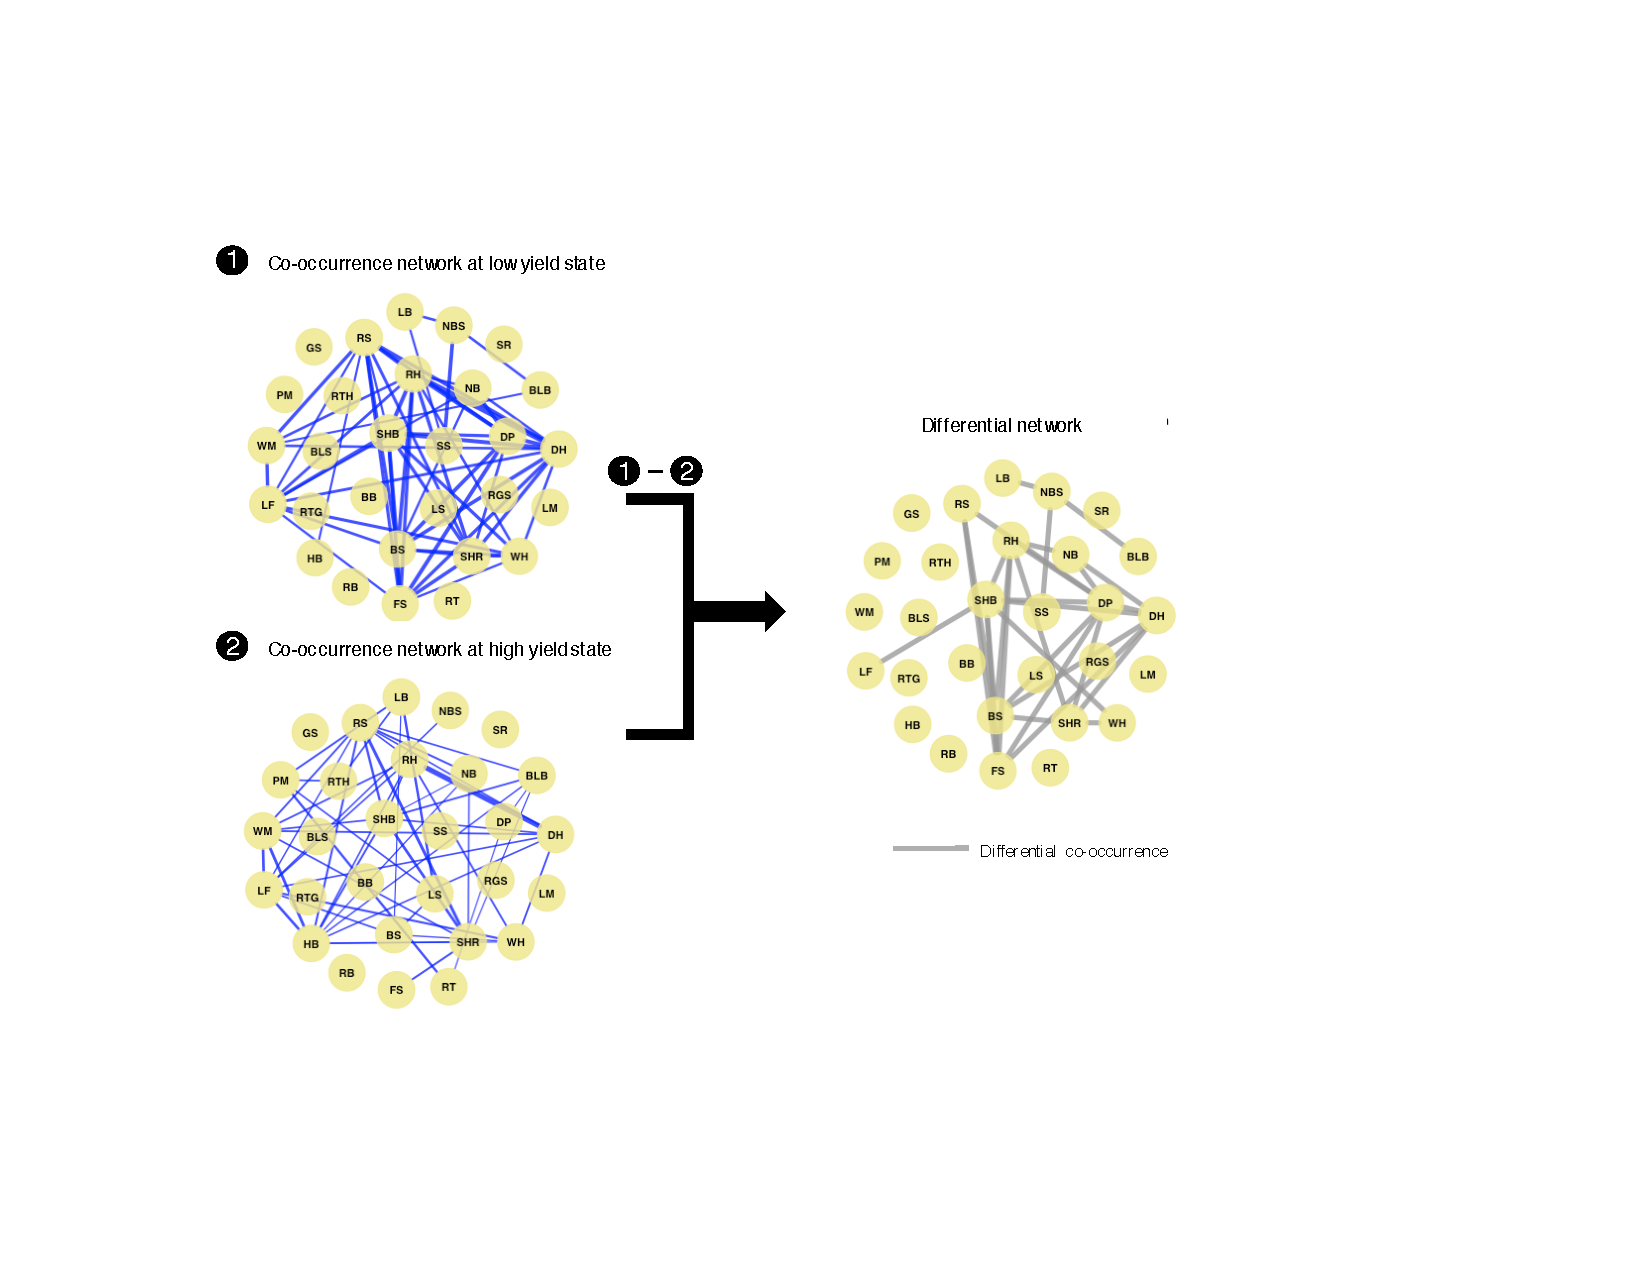
\includegraphics[width = 1\textwidth]{figures/pipeline4.pdf}
\caption[Differential analysis of crop health survey data at different yield levels]{Schematic showing differential analysis at different yield levels. Co-occurrence networks are measured in each of two different yield levels (left) resulting in interactions (blue). The network at low yield level network is subtracted from high yield level to create a differential co-occurrence network (right), in which the significant differential interactions are those that positive in score after the shift from low to high yield state.}
\label{fig:pipeline4}
\end{figure} 

\textbf{Topological properties}
To investigate the structural properties of differential networks, I calculated topological features for each node in the network with the \textbf{igraph} package. This feature set included node degree, clustering coefficient, and betweenness. 


\clearpage
\subsection{Results}

Differential network approach to constructing response networks enables easy comparison of the generated graphs. This, in turn allowed identification of the differences between the responses of co-occurrence relationships of rice injuries. In particular, in the differential network, I identified injuries and network components that are relevant for responsive condition as well as responsible for condition. 


\subsubsection{Construction of differential co-occurrence networks of rice injuries at different seasons}

I determined differential co-occurrence patterns of rice injuries of survey data in dry and wet season. The Differential co-occurrence network in season (DCONS), presenting pairs of injuries (nodes) connected with significantly different co-occurrence relationships (edges), are showed in \ref{fig:difseasonCP} - \ref{fig:difseasonWJ}. DCONS at Central Plain (Figure. \ref{fig:difseasonCP}) reveals SHB, SHR, and RS showing significantly different co-occurrence in both dry and wet season. They are likely to observed theses injuries. DP, SHB are high-betweenness in this network. Obviously, DP are likely to be observed in dry season because there are many pathway to increase it. Also, SHB  


   var degree betweenness clust.coef
1   RH      1    0.000000        NaN
2   SS      1    0.000000        NaN
3   WH      3    1.750000  0.0000000
4   DH      1    0.000000        NaN
5   DP      8   36.750000  0.1428571
6   FS      4    4.750000  0.5000000
7   NB      1    0.000000        NaN
8   WM      1    0.000000        NaN
9  BLB      2    0.250000  0.0000000
10  BS      3    4.333333  0.3333333
11  LB      1    0.000000        NaN
12  RS      4    6.833333  0.1666667
13  HB      1    0.000000        NaN
14 SHB      5   21.500000  0.2000000
15 SHR      4    6.833333  0.1666667


DCONS at OD \ref{fig:difseasonOD} reveals LB different both in dry and wet season. The group of injuries that present in wet season are RH, SS, FS, DH, and LM. But in dry season, there are SHB, BS, WH, NB.

var degree betweenness clust.coef
1   RH      2         0.0  1.0000000
2   SS      3         0.5  0.6666667
3   DH      2         0.0  1.0000000
4   FS      3         0.5  0.6666667
5   NB      1         0.0        NaN
6   LM      1         0.0        NaN
7   WM      1         0.0        NaN
8   BS      2         1.0  0.0000000
9   LB      2         1.0  0.0000000
10 SHB      1         0.0        NaN

DCONS at RR \ref{fig:difseasonRR} reveals that DP, BS, RTH, LF. 

PM- NBS in wet season , GS-BB-BLS in dry season

var degree betweenness clust.coef
1   WH      2          12          0
2   PM      1           0        NaN
3   DP      2          12          0
4  RTH      2           6          0
5   LF      2           6          0
6   WM      1           0        NaN
7  BLB      2          10          0
8  BLS      1           0        NaN
9   BS      2          10          0
10  LB      1           0        NaN
11 NBS      1           0        NaN
12  BB      1           0        NaN
13  GS      2           1          0

DCONS at TM shows two injury pairs express significantly co-occurrence in dry season, which are WH-BS, and DP-RTH, and one injury pair (SHB-LF) apparently occur together in wet season. 



DCONS at WJ (Figure.\ref{fig:difseasonnetwork_WJ} revealed that BS, NBS, SHB, and BLS co-occurring in both seasons.   

There are cluster group of injuries PM RS RTG RGS BB GS in dry season 

DP SHR

\ref{fig:difseasonTM}
   var degree betweenness clust.coef
1   RT      2   0.3333333  0.0000000
2   RH      3   5.6666667  0.0000000
3   WH      1   0.0000000        NaN
4   PM      5   0.2500000  0.9000000
5   RB      1   0.0000000        NaN
6   DH      3   5.6666667  0.0000000
7   DP      6   7.7500000  0.4666667
8   NB      1   0.0000000        NaN
9   LF      3   0.0000000  1.0000000
10  LM      1   0.0000000        NaN
11  LS      1   0.0000000        NaN
12  WM      2   0.5000000  0.0000000
13 BLB      3   1.0000000  0.6666667
14 BLS      4   4.8333333  0.1666667
15  BS      4   7.7500000  0.5000000
16 NBS      2   2.2500000  0.0000000
17  RS      4   0.0000000  1.0000000
18  BB      4   0.0000000  1.0000000
19  GS      5   0.2500000  0.9000000
20 RGS      5   0.2500000  0.9000000
21 RTG      5   0.2500000  0.9000000
22 SHB      7  27.1666667  0.2380952
23 SHR      6  14.0833333  0.4000000




\subsection{shared co-occurrence patterns networks of rice injuries at different season}

\begin{figure}
\centering
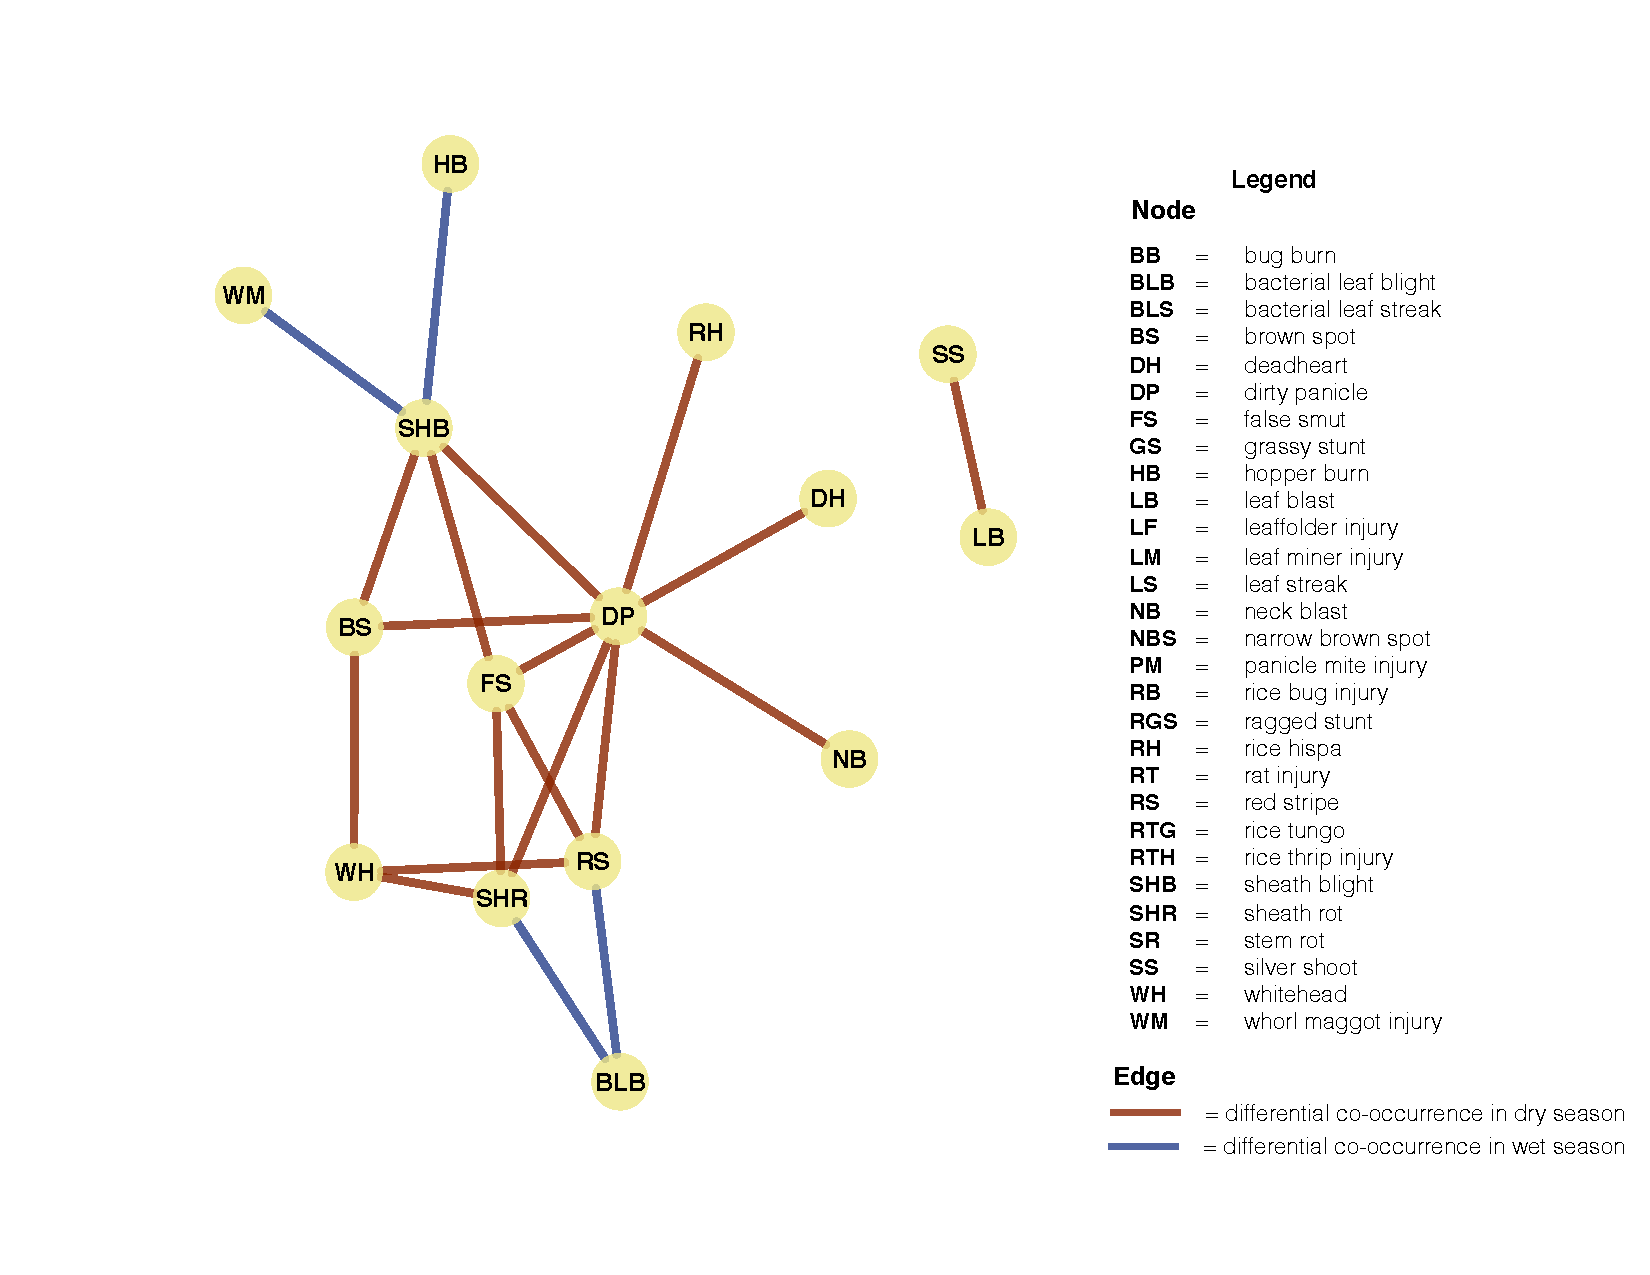
\includegraphics[width = 1\textwidth]{figures/difseasonCP.pdf}
\caption{Differential co-occurrence network of rice injuries in different seasons at Central Plain, Thailand}
\label{fig:difseasonnetwork_CP}
\end{figure} 

\begin{figure}
\centering
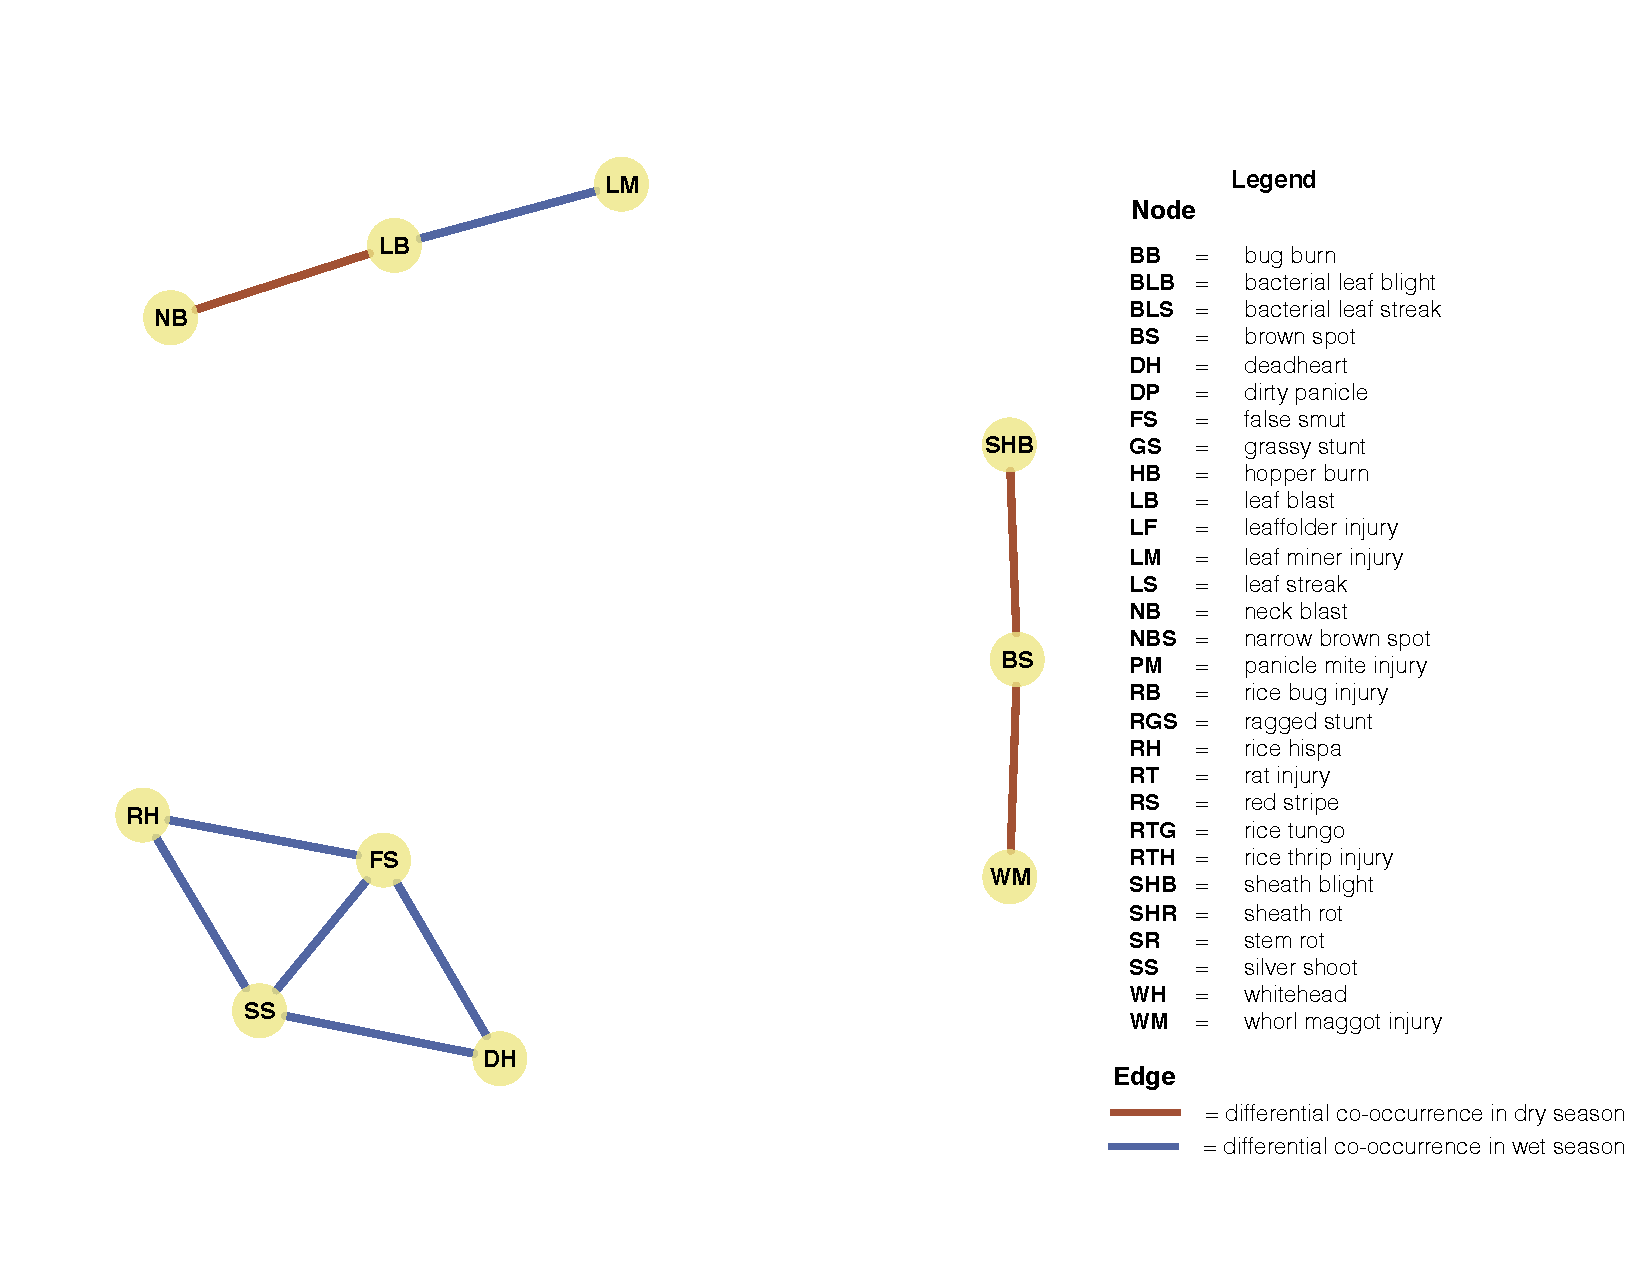
\includegraphics[width = 1\textwidth]{figures/difseasonOR.pdf}
\caption{Differential co-occurrence network of rice injuries in different seasons at Odisha, India }
\label{fig:difseasonnetwork_OR}
\end{figure}


\begin{figure}
\centering
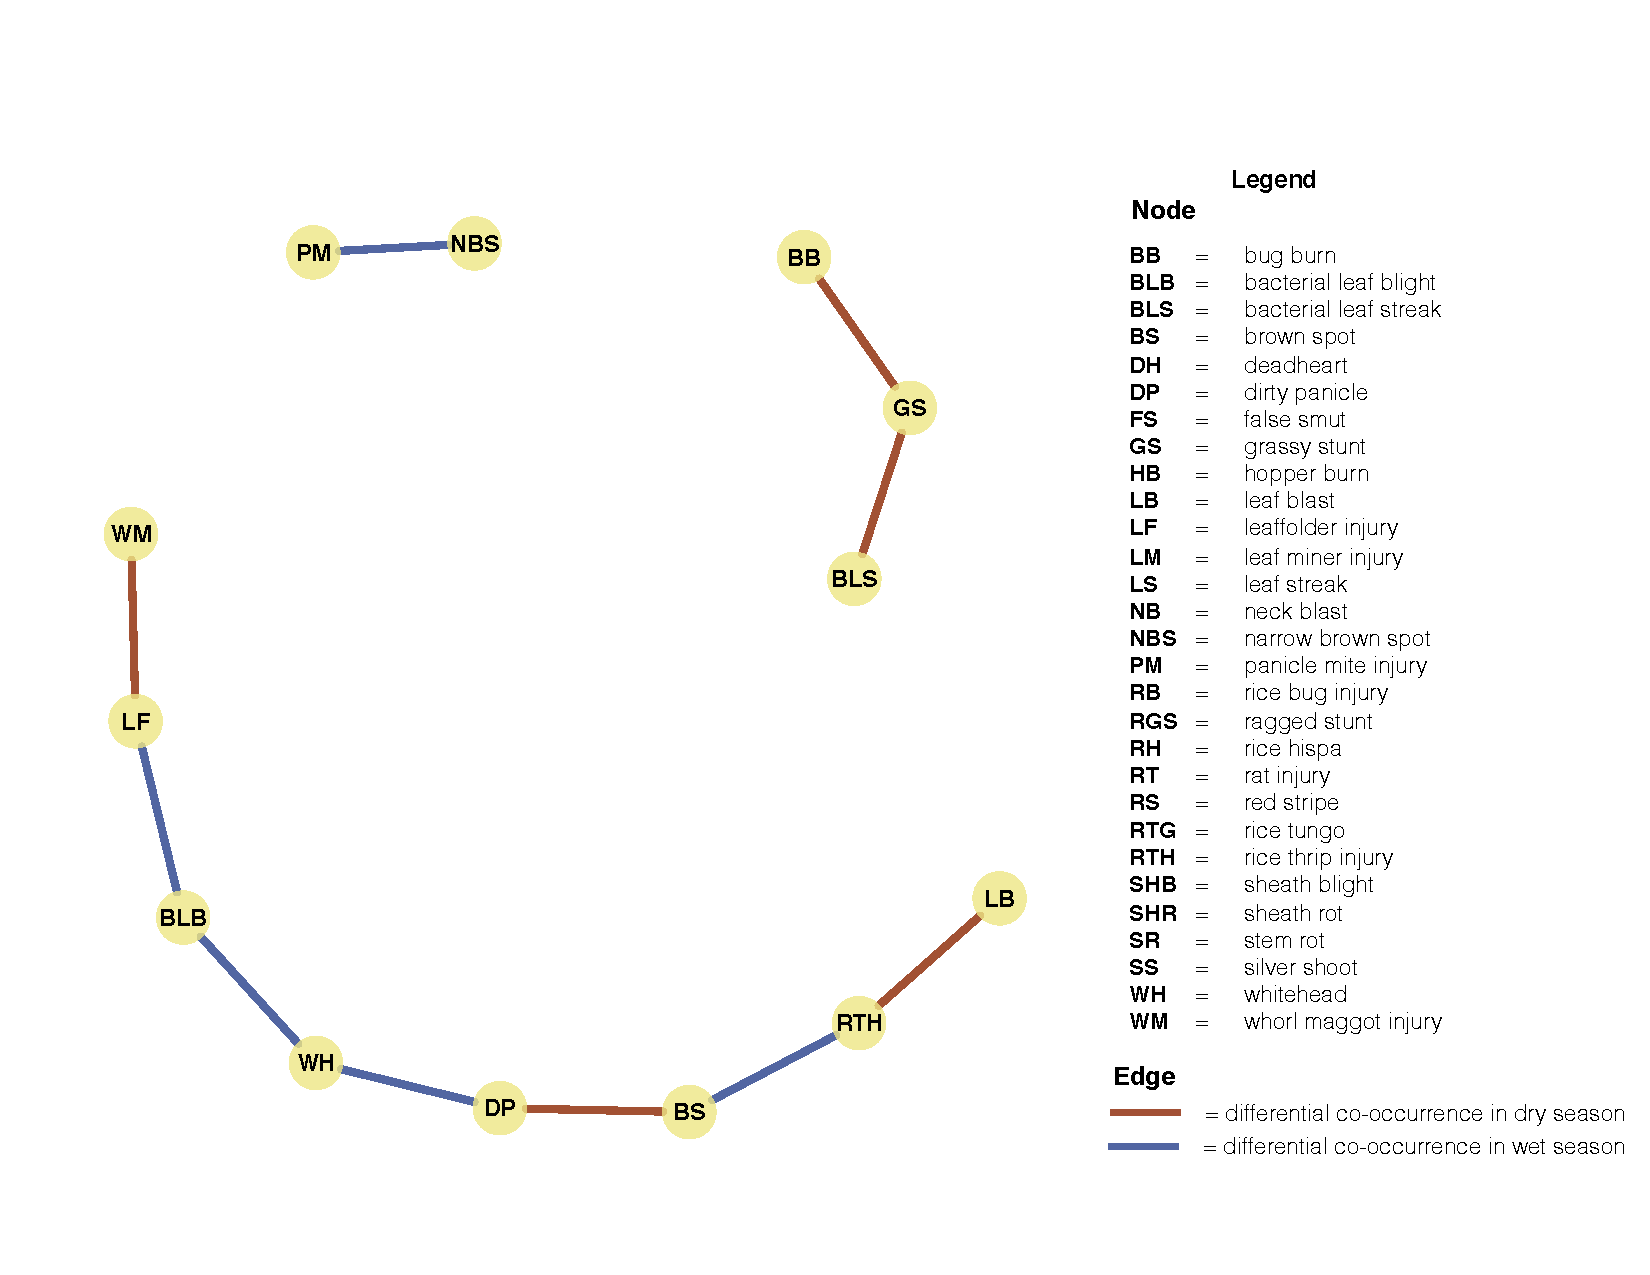
\includegraphics[width = 1\textwidth]{figures/difseasonRR.pdf}
\caption{Differential co-occurrence network of rice injuries in different seasons at Red River Delta, Vietnam}
\label{fig:difseasonnetwork_RR}
\end{figure}


\begin{figure}
\centering
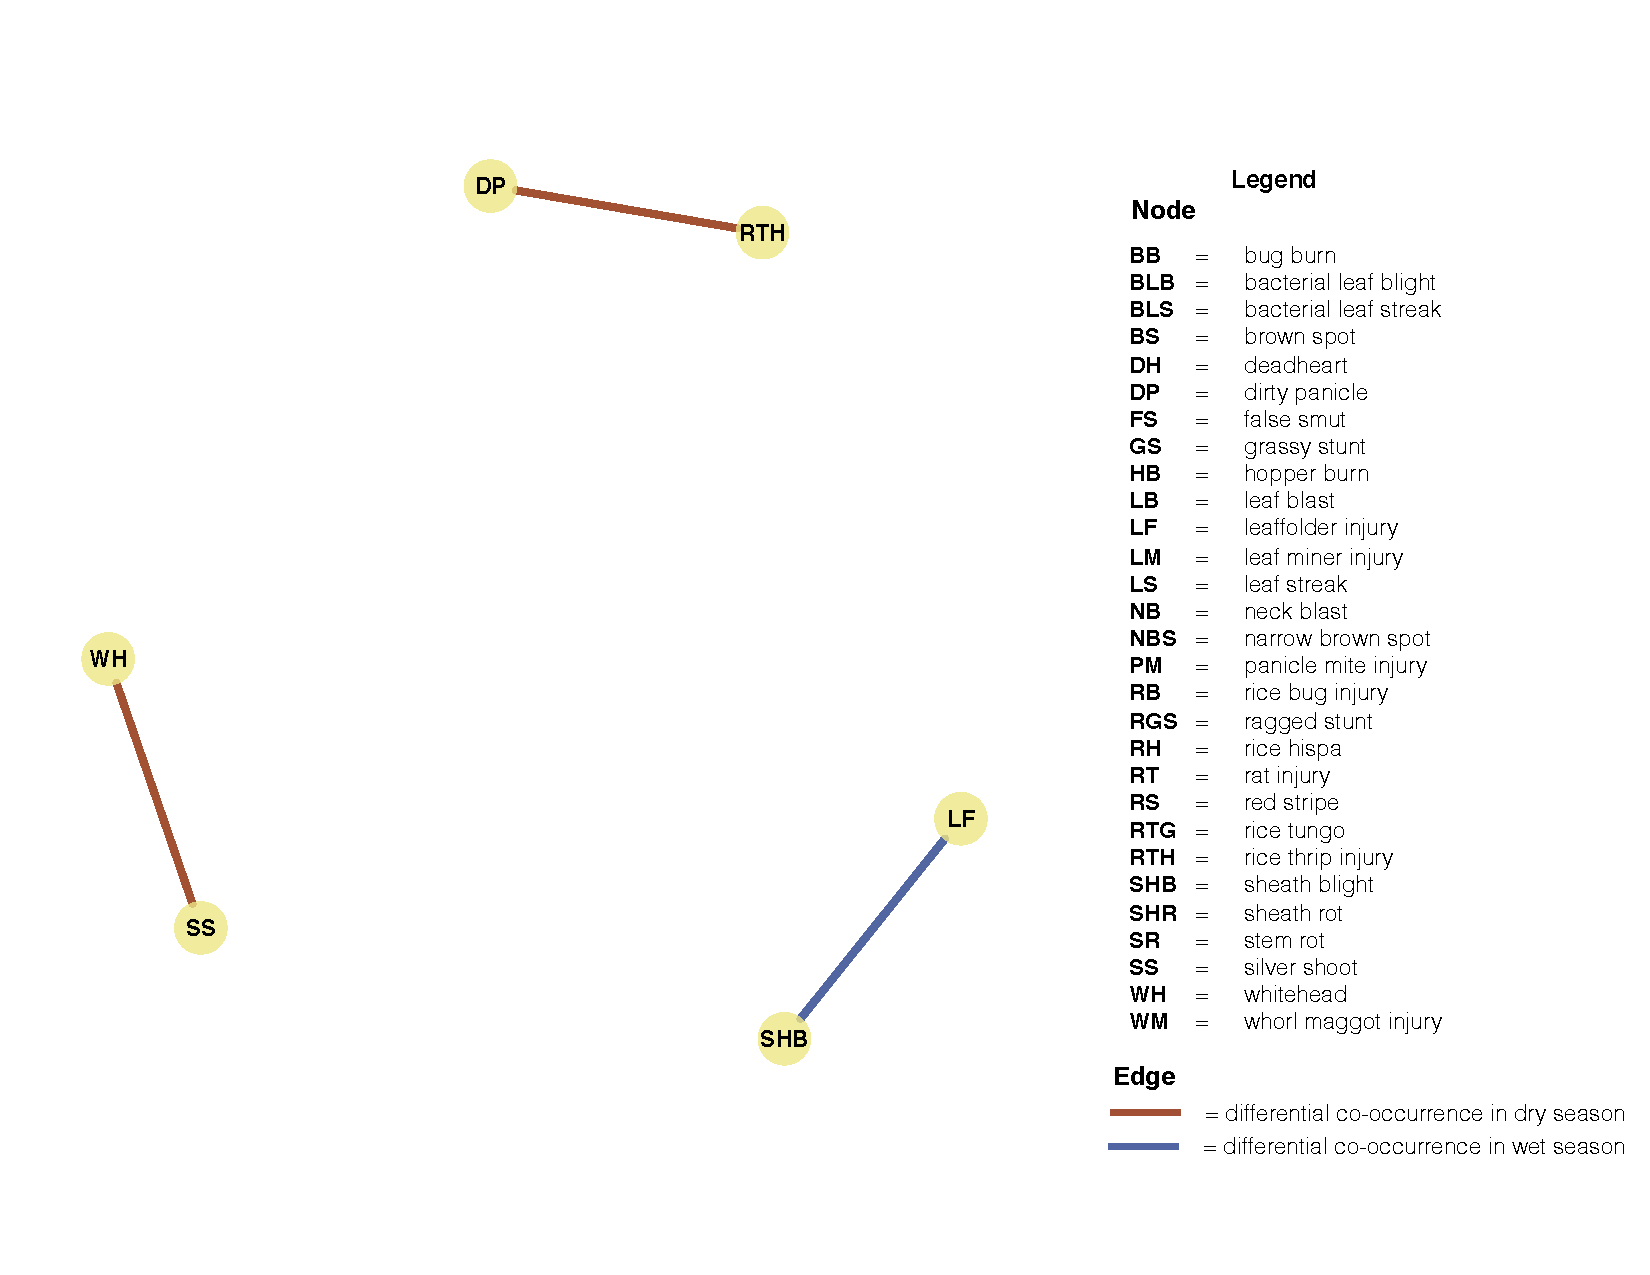
\includegraphics[width = 1\textwidth]{figures/difseasonTM.pdf}
\caption{Differential co-occurrence network of rice injuries in different seasons at Tamil Nadu, India}
\label{fig:difseasonTM}
\end{figure}


\begin{figure}
\centering
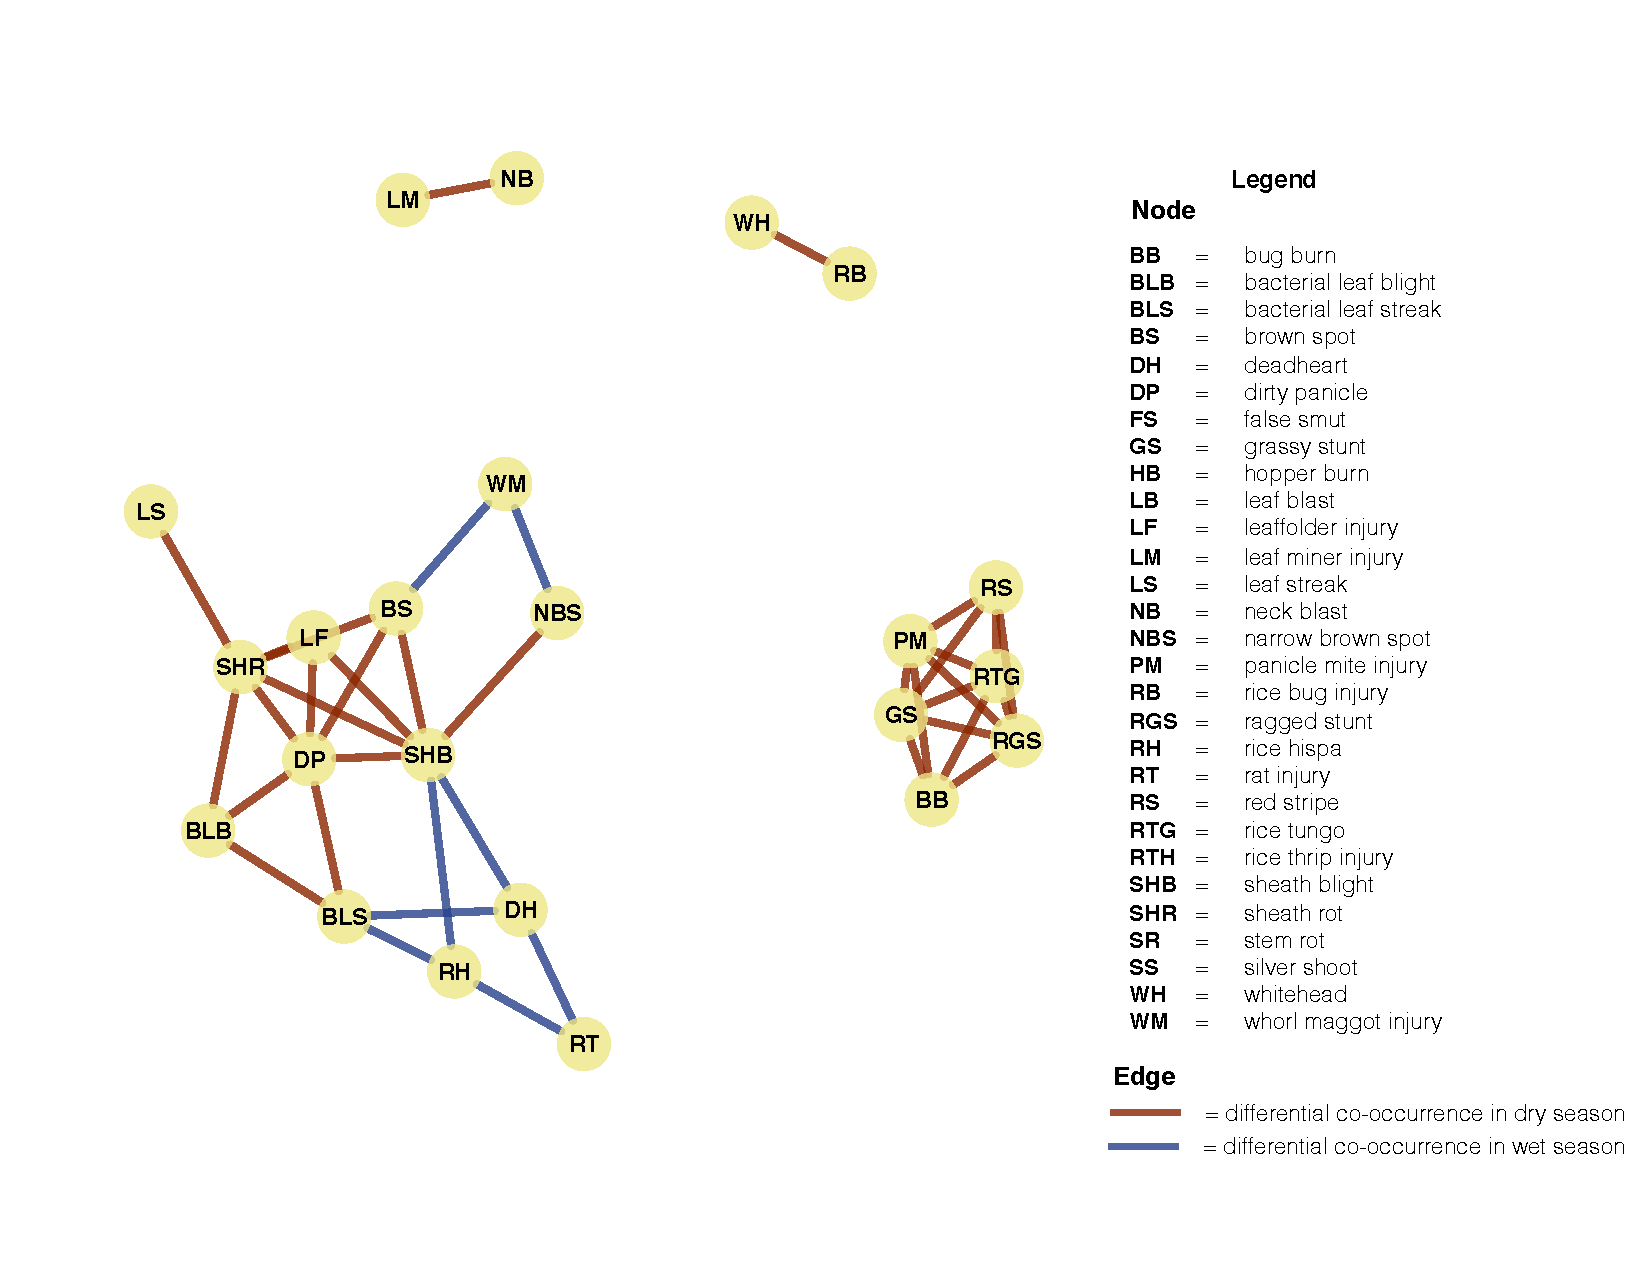
\includegraphics[width = 1\textwidth]{figures/difseasonWJ.pdf}
\caption{Differential co-occurrence network of rice injuries in different seasons at West Java, Indonesia}
\label{fig:difseasonWJ}
\end{figure}

%================================
\subsubsection{Differential co-occurrence networks of rice injuries at yield levels}

Comparison of the injury co-occurrence networks differed by season and the generic stress response network induced by different yield levels revealed features unique to each graph. In particular, I not only detected the presence of injuries, but I was able to see how they interacted with other genes in their respective networks. 
The injuries showed in the differential networks are the injuries showed co-occurrence patterns represented by edges. Edges were determined as co-occurrence correlation that express significantly higher in lower yield level. 

In this study, three successive yield classes were defined, in order to enable a better description of actual yield, from low (< 4 ton/ha), medium (4 – 6 ton/ha),  high (> 6 ton/ha) yield levels. Figure \ref{fig:yield_level_bar} shows the number of farmers’ fields surveyed classified in each season, and production environment.

\citet{Berry_2014_Deciphering} recommended that a co-occurrence network will be more reliable, it should be produced using a minimum of 25 samples or observations. From figure \ref{fig:yield_level_bar}, to be able compare the networks at different yield levels, I chose the data set, which are medium and high yield level of Central Plain, low and medium yield level of Odisha, medium and high yield level at Red River Delta, low and medium yield level of Tamil Nadu, and medium and high yield level of West Java. 

The resulted networks, differential co-occurrence network in yield (DCON-Y), depicts the associations of injury pairs significantly expressing in lower yield state but absent in higher yield state. Figures.\ref{fig:difyieldnetwork_CP} presents DCON-Y between medium and high yield level. It comprised of two groups of related injuries. Form node properties, DP, SHB, BS, RH, FS, and DH are high node degree and betweenness, which are likely to occur in this state because there are many connection, which can increase other injuries related, be induced by them as well. BS, SHB, are DP recorded in survey data showed these injuries were observed higher in medium than high yield data set(Fiure. \ref{fig:nodepropdifyield_CP}). DCON-Y compared between low yield and medium yield level at Odisha (Figure \ref{fig:difyieldnetwork_OD}) shows closely associated injures (DH, RH, FS, BS, WH). Their relationships were captured only in low yield state, and WH, BS, and FS are injuries connecting to all the injuries. Survey data also found that these injuries were observed in high frequency at high level of incidence (Figure \ref{fig:nodepropdifyield_OD}). In Red River delta, DCON-Y (Figure.\ref{fig:difyieldnetwork_RR}) reveals three injury combinations (DP-WH, GS-BB, and WM-LB-RTH) presenting in medium yield level, not in high yield level. So their co-occurrences may affect to yield losses between medium to high yield levels. Based on the survey data, DP, WM, and WH were found more incidence in low yield than high yield level (Figure. \ref{fig:nodepropdifyield_RR}). Apparently, in Tamil Nadu, Figure.\ref{fig:difyieldnetwork_TM} showed the co-occurrence pattern between SHB and WH that was found only in low yield level state, even though, from survey data, WH were found higher incidence in medium yield level than low yield level, but SHB were observe high incidence in low yield level than medium yield level (Figure \ref{nodepropdifyieldnetwork_TM}). In West Java, DCONY (Figure. \ref{fig:difyieldnetwork_TM}) reveals two groups of associated injuries that significantly express in medium yield level state. Form topological features of this DCON-Y, FS, RS, SHB, and LB are high betweenness nodes, which they are more likely to occur or be observed in this state because there are many pathway to increase them. SHB based on survey data also were highly found in medium than high yield level (Figure.\ref{fig:nodepropdifyield_WJ}).  

\begin{figure}
    \centering
        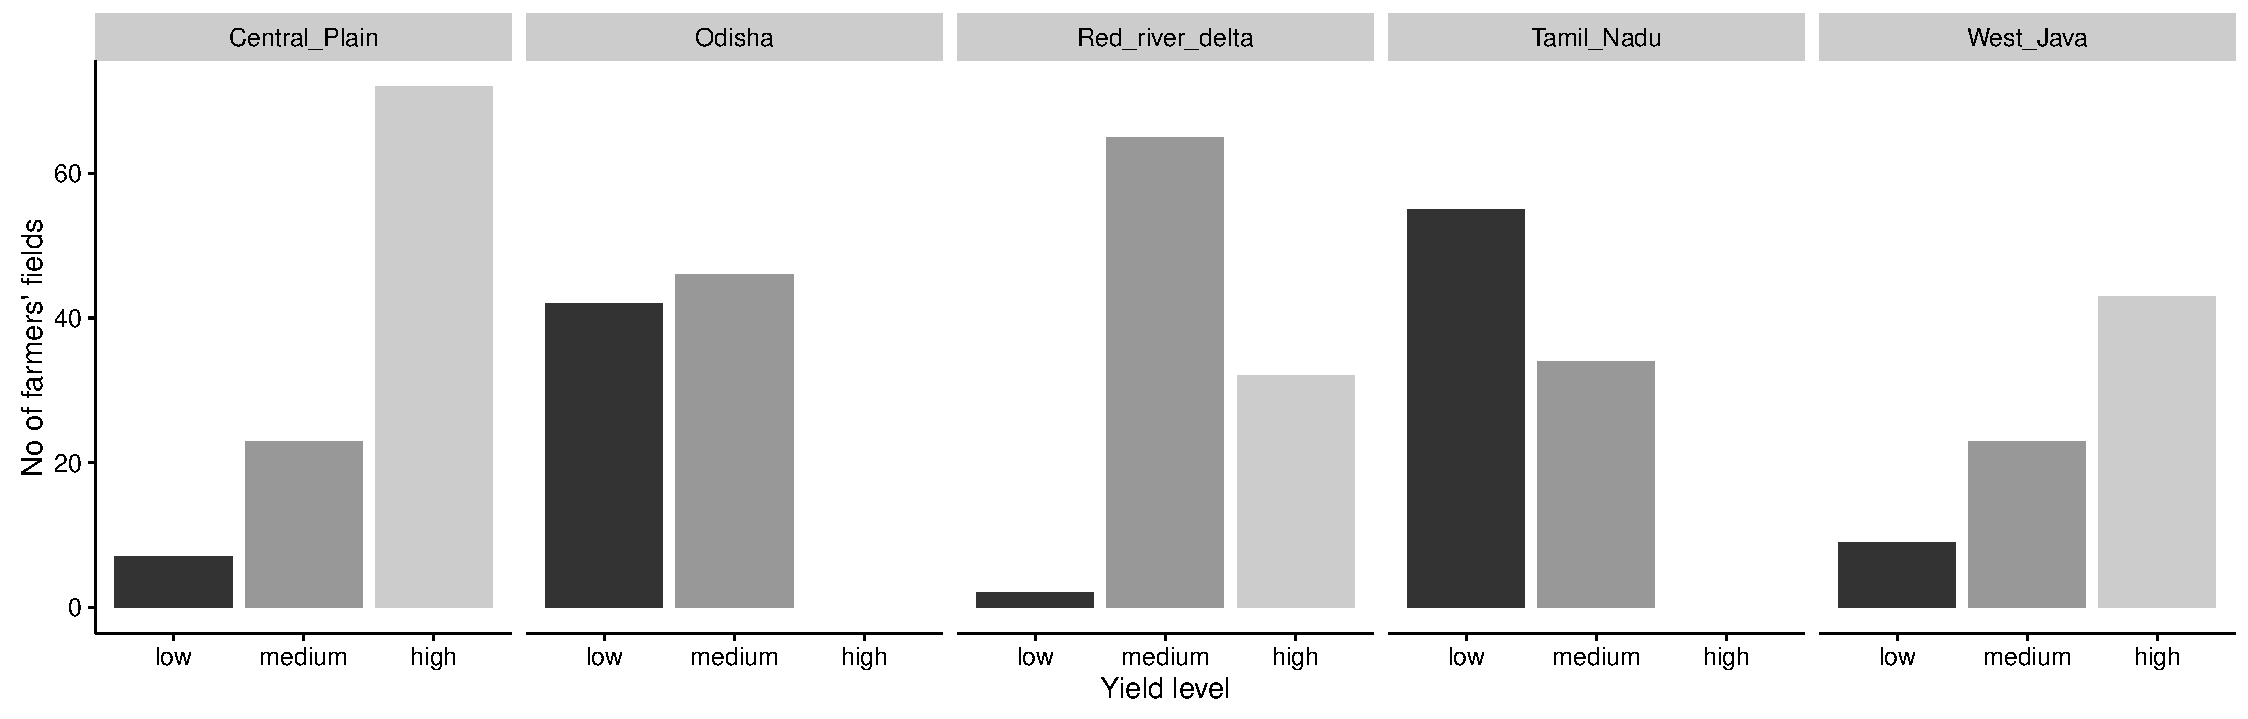
\includegraphics[width = 1\textwidth]{figures/yield_level_bar.pdf}
\caption{Bar graphs showing number of farmers' fields classified by different yield levels in each production environment.}
\label{fig:yield_level_bar}
\end{figure}

\begin{figure}
    \centering
    \begin{subfigure}[b]{1\textwidth}
        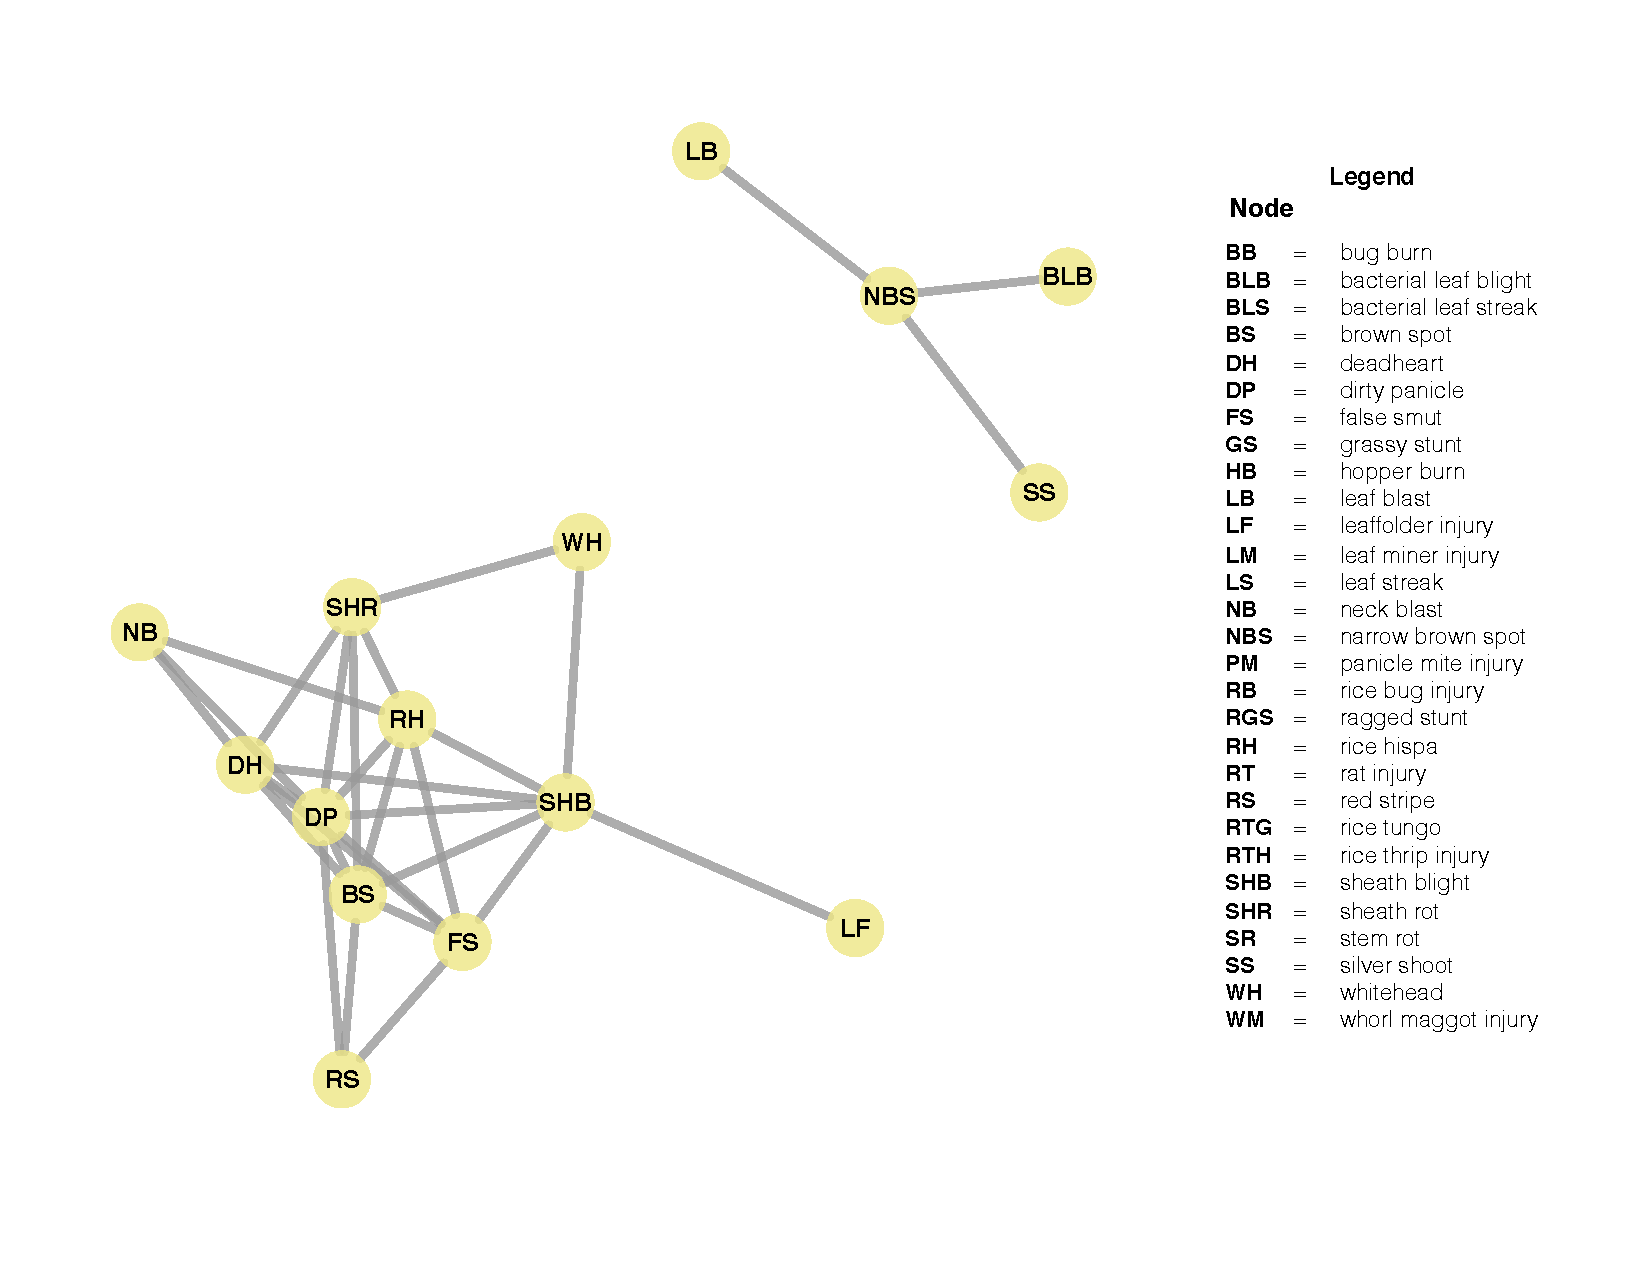
\includegraphics[width = 0.9\textwidth]{figures/difyieldCP.pdf}
        \caption[Differential co-occurrence network of rice injuries in different yield levels at Central Plain, Thailand]{Differential co-occurrence network of rice injuries in different yield levels at Central Plain, Thailand. The layout of the network graph is based on the Fruchterman-Reingold algorithm, which places nodes with stronger or more connections closer to each other.}
        \label{fig:difyieldnetwork_CP}
    \end{subfigure}
    \begin{subfigure}[b]{0.9\textwidth}
        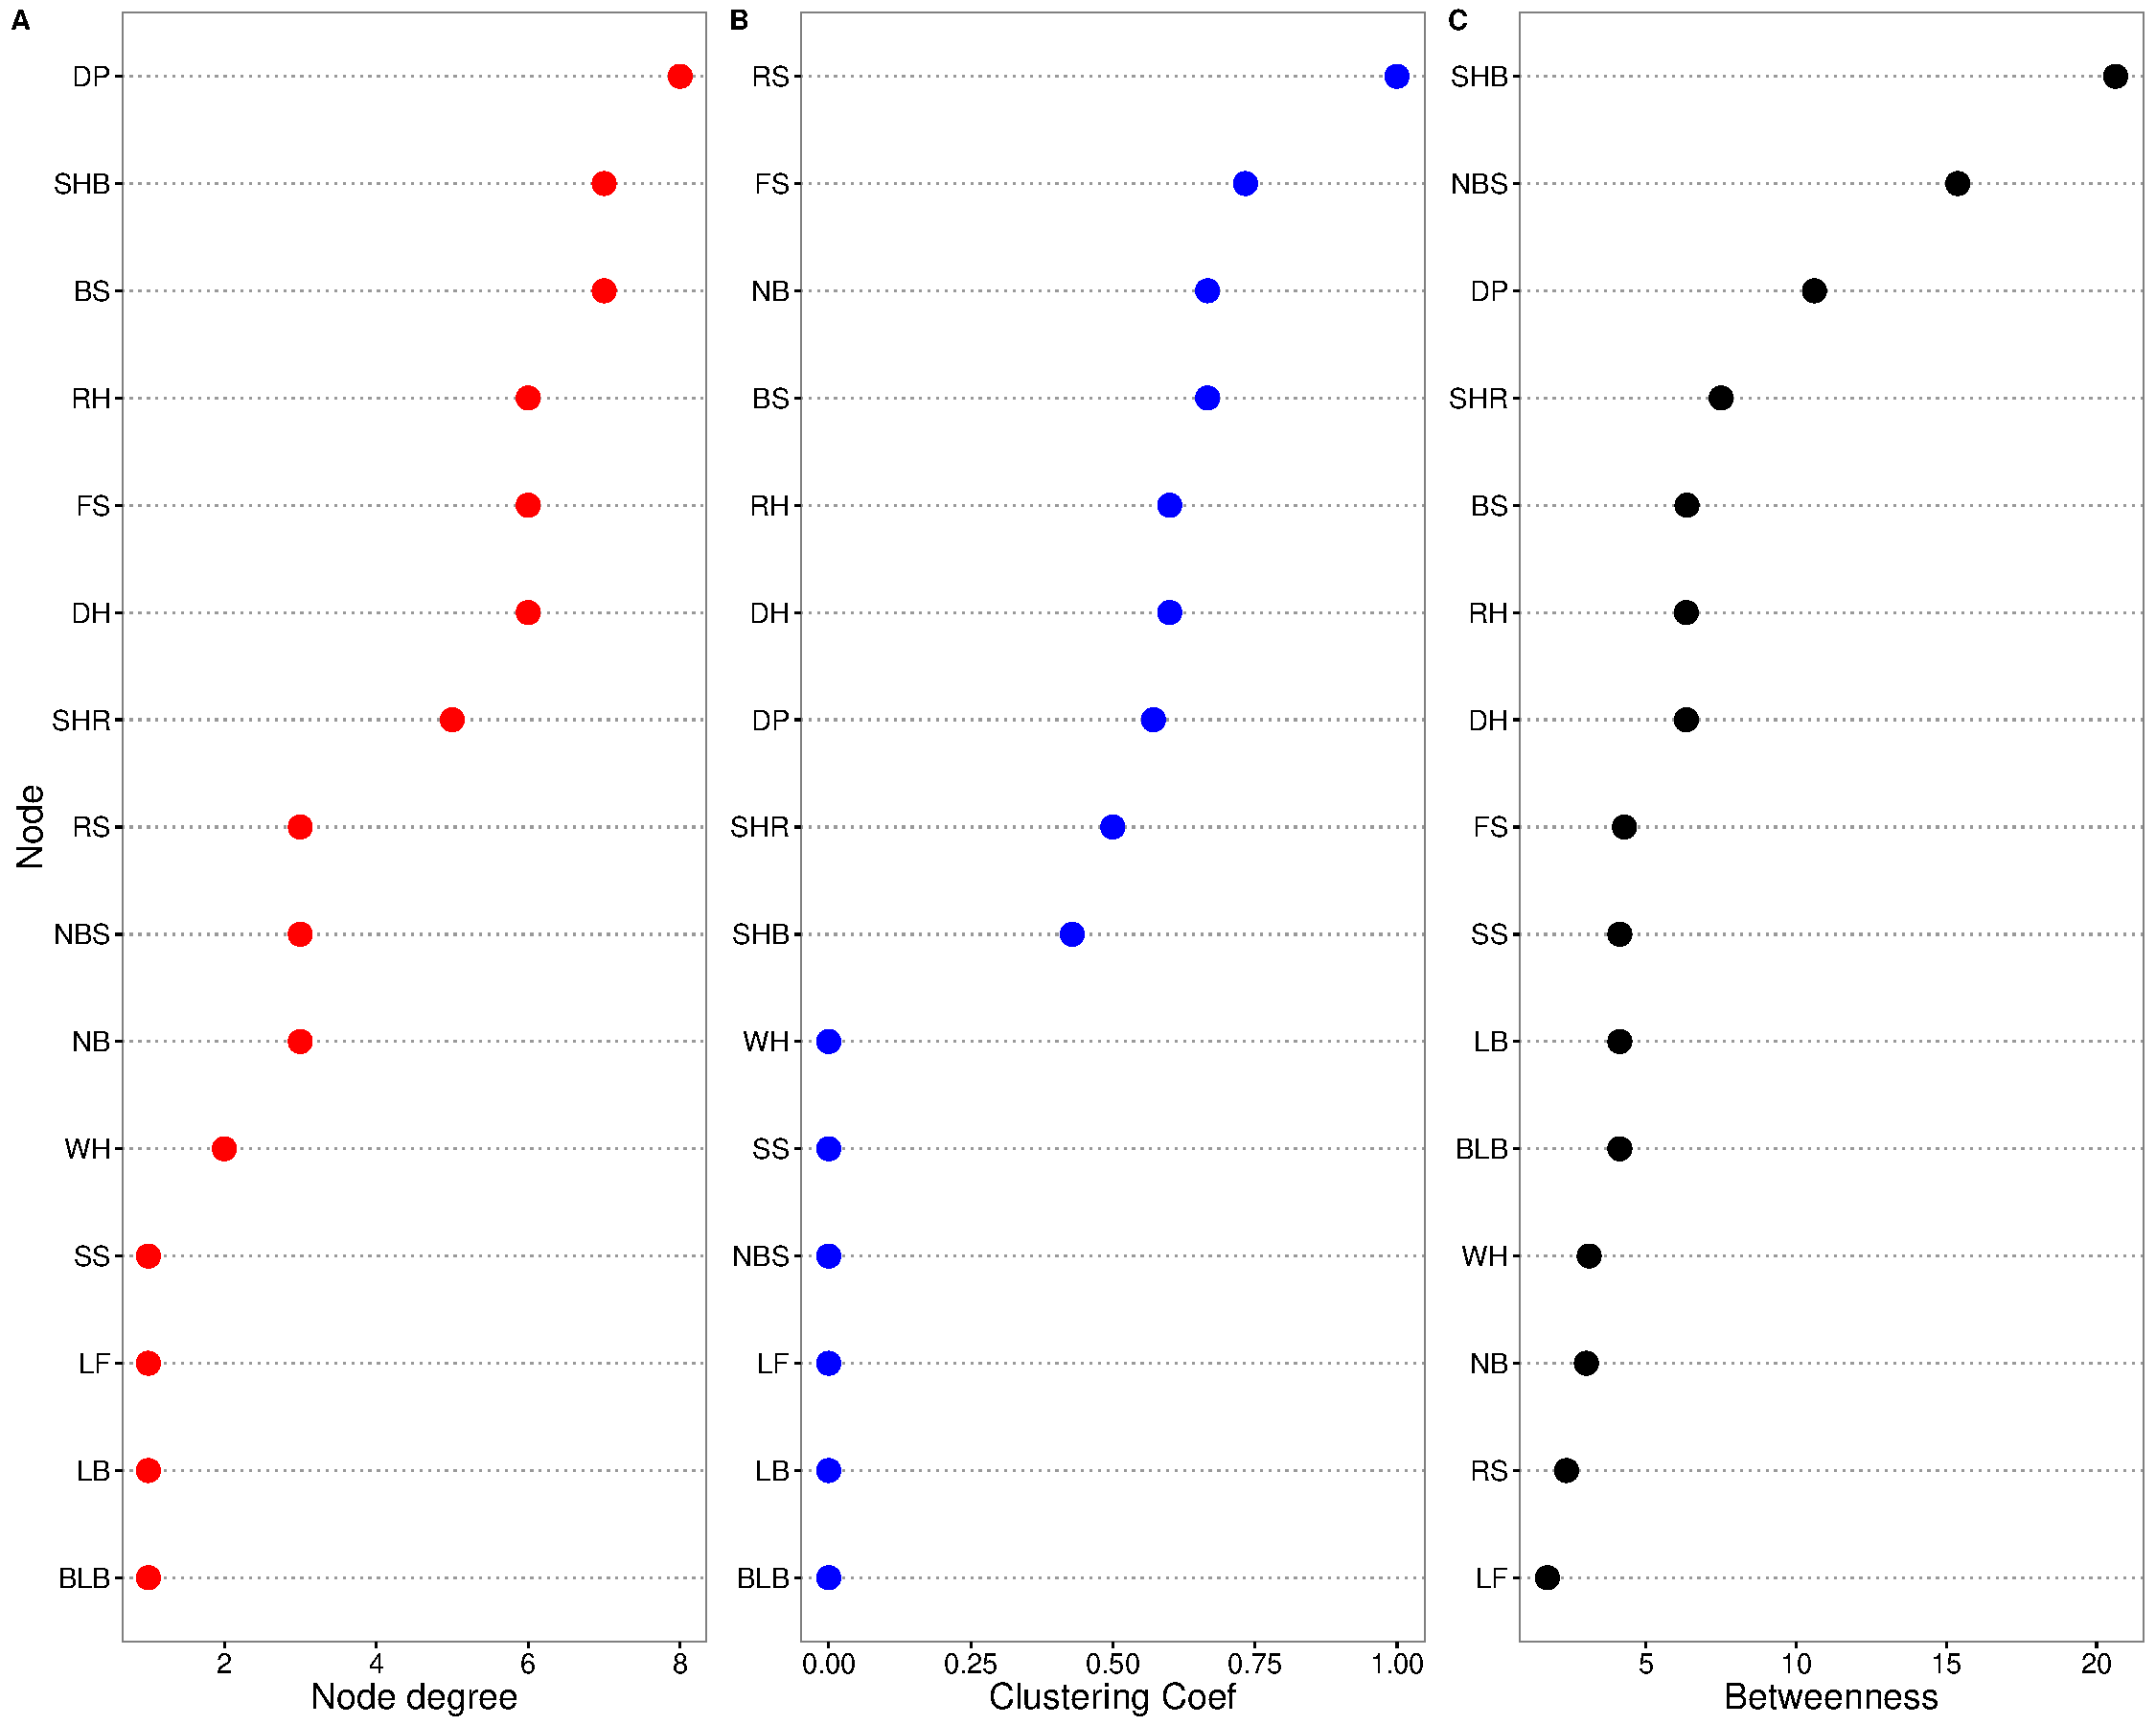
\includegraphics[width = 1\textwidth]{figures/yield_dif_nodepropCentral_Plain.pdf}
        \caption[Three centrality measures of the nodes in co-occurrence network of rice injuries in dry season at Central Plain.]{Three centrality measures of the nodes in co-occurrence network of rice injuries in dry season at Central Plain. A: node degree, B:clustering coefficient, and C:Betweenness.}
        \label{fig:nodepropdifyield_CP}
    \end{subfigure}
    \caption{Differential network analysis of survey data in different yield levels at Central Plain, Thailand.}
    \label{fig:difyield_CP}
\end{figure}
 
\begin{figure}
    \centering
    \begin{subfigure}[b]{1\textwidth}
        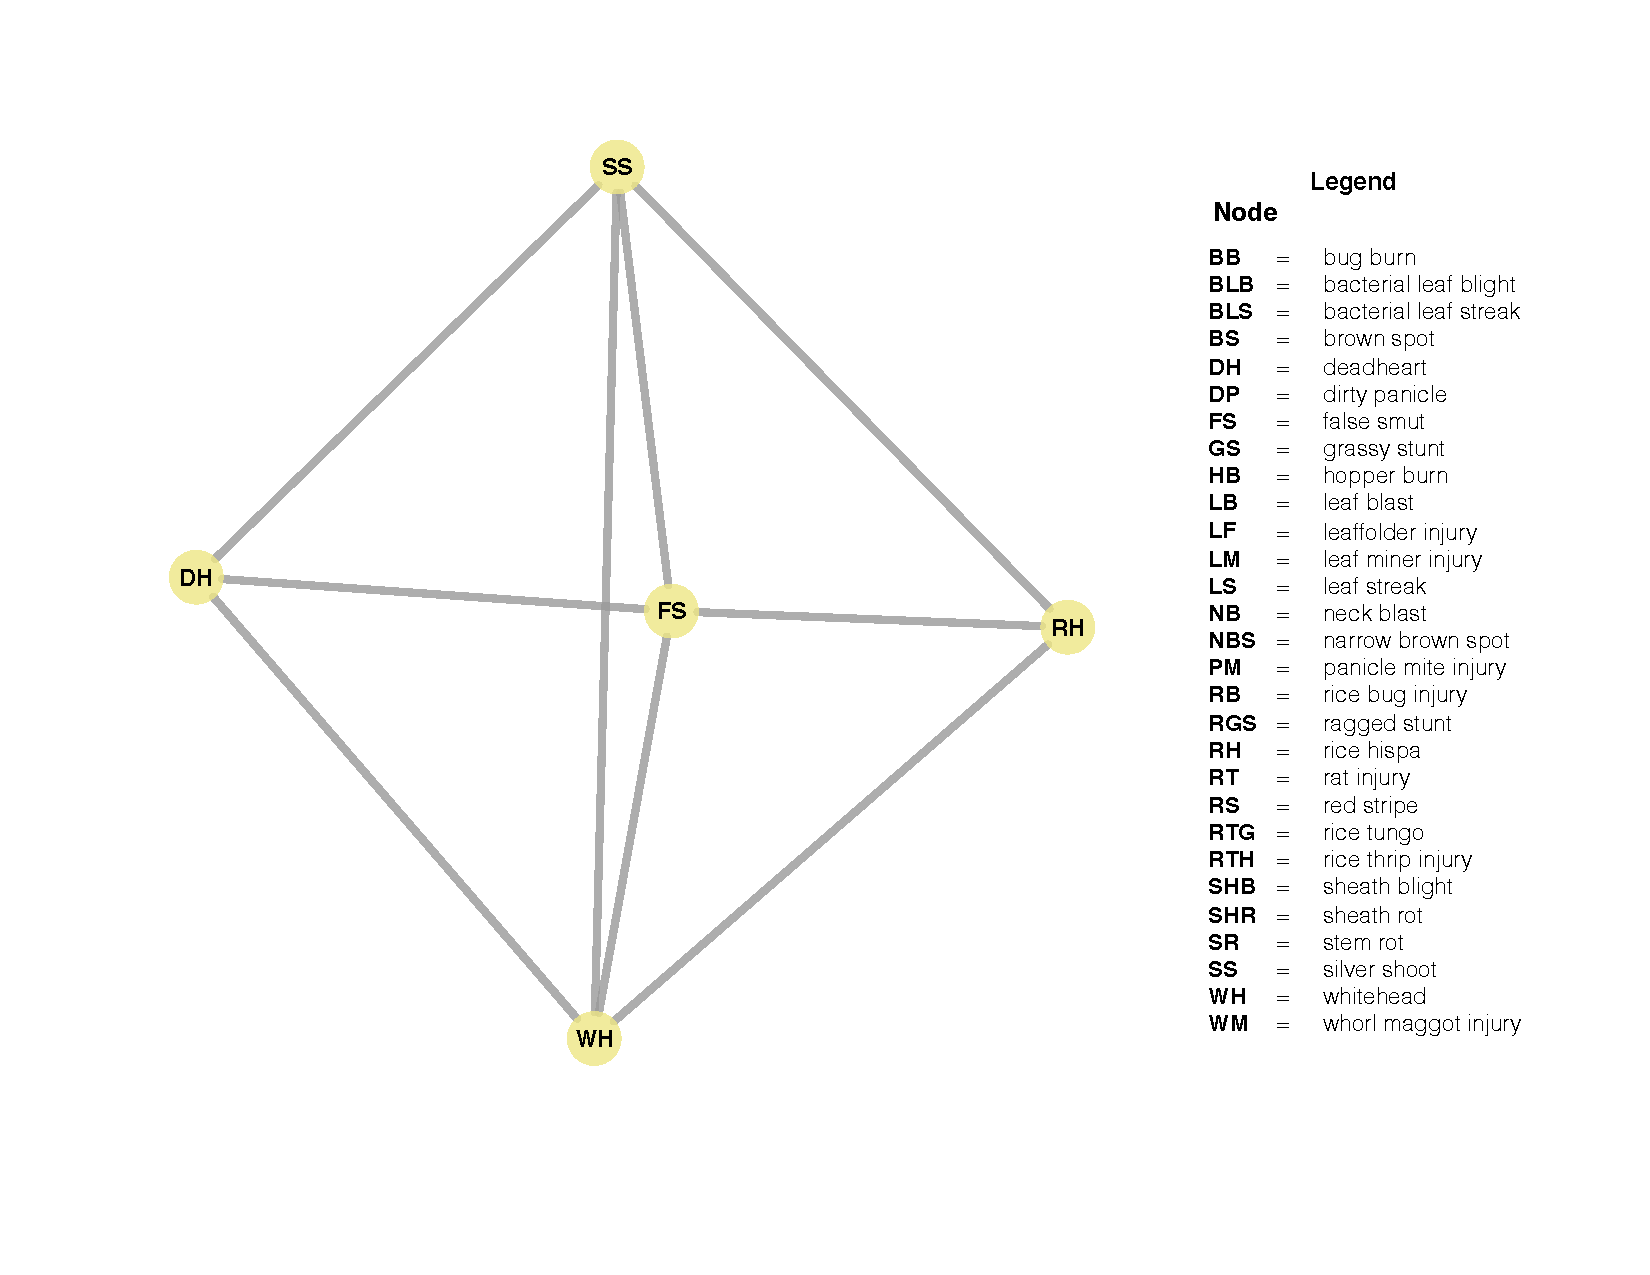
\includegraphics[width = 1\textwidth]{figures/difyieldOD.pdf}
        \caption[Differential co-occurrence network of rice injuries in different yield levels at Odisha, India.]{Differential co-occurrence network of rice injuries in different yield levels at Odisha, India. The layout of the network graph is based on the Fruchterman-Reingold algorithm, which places nodes with stronger or more connections closer to each other.}
        \label{fig:difyieldnetwork_OD}
    \end{subfigure}
    \begin{subfigure}[b]{1\textwidth}
        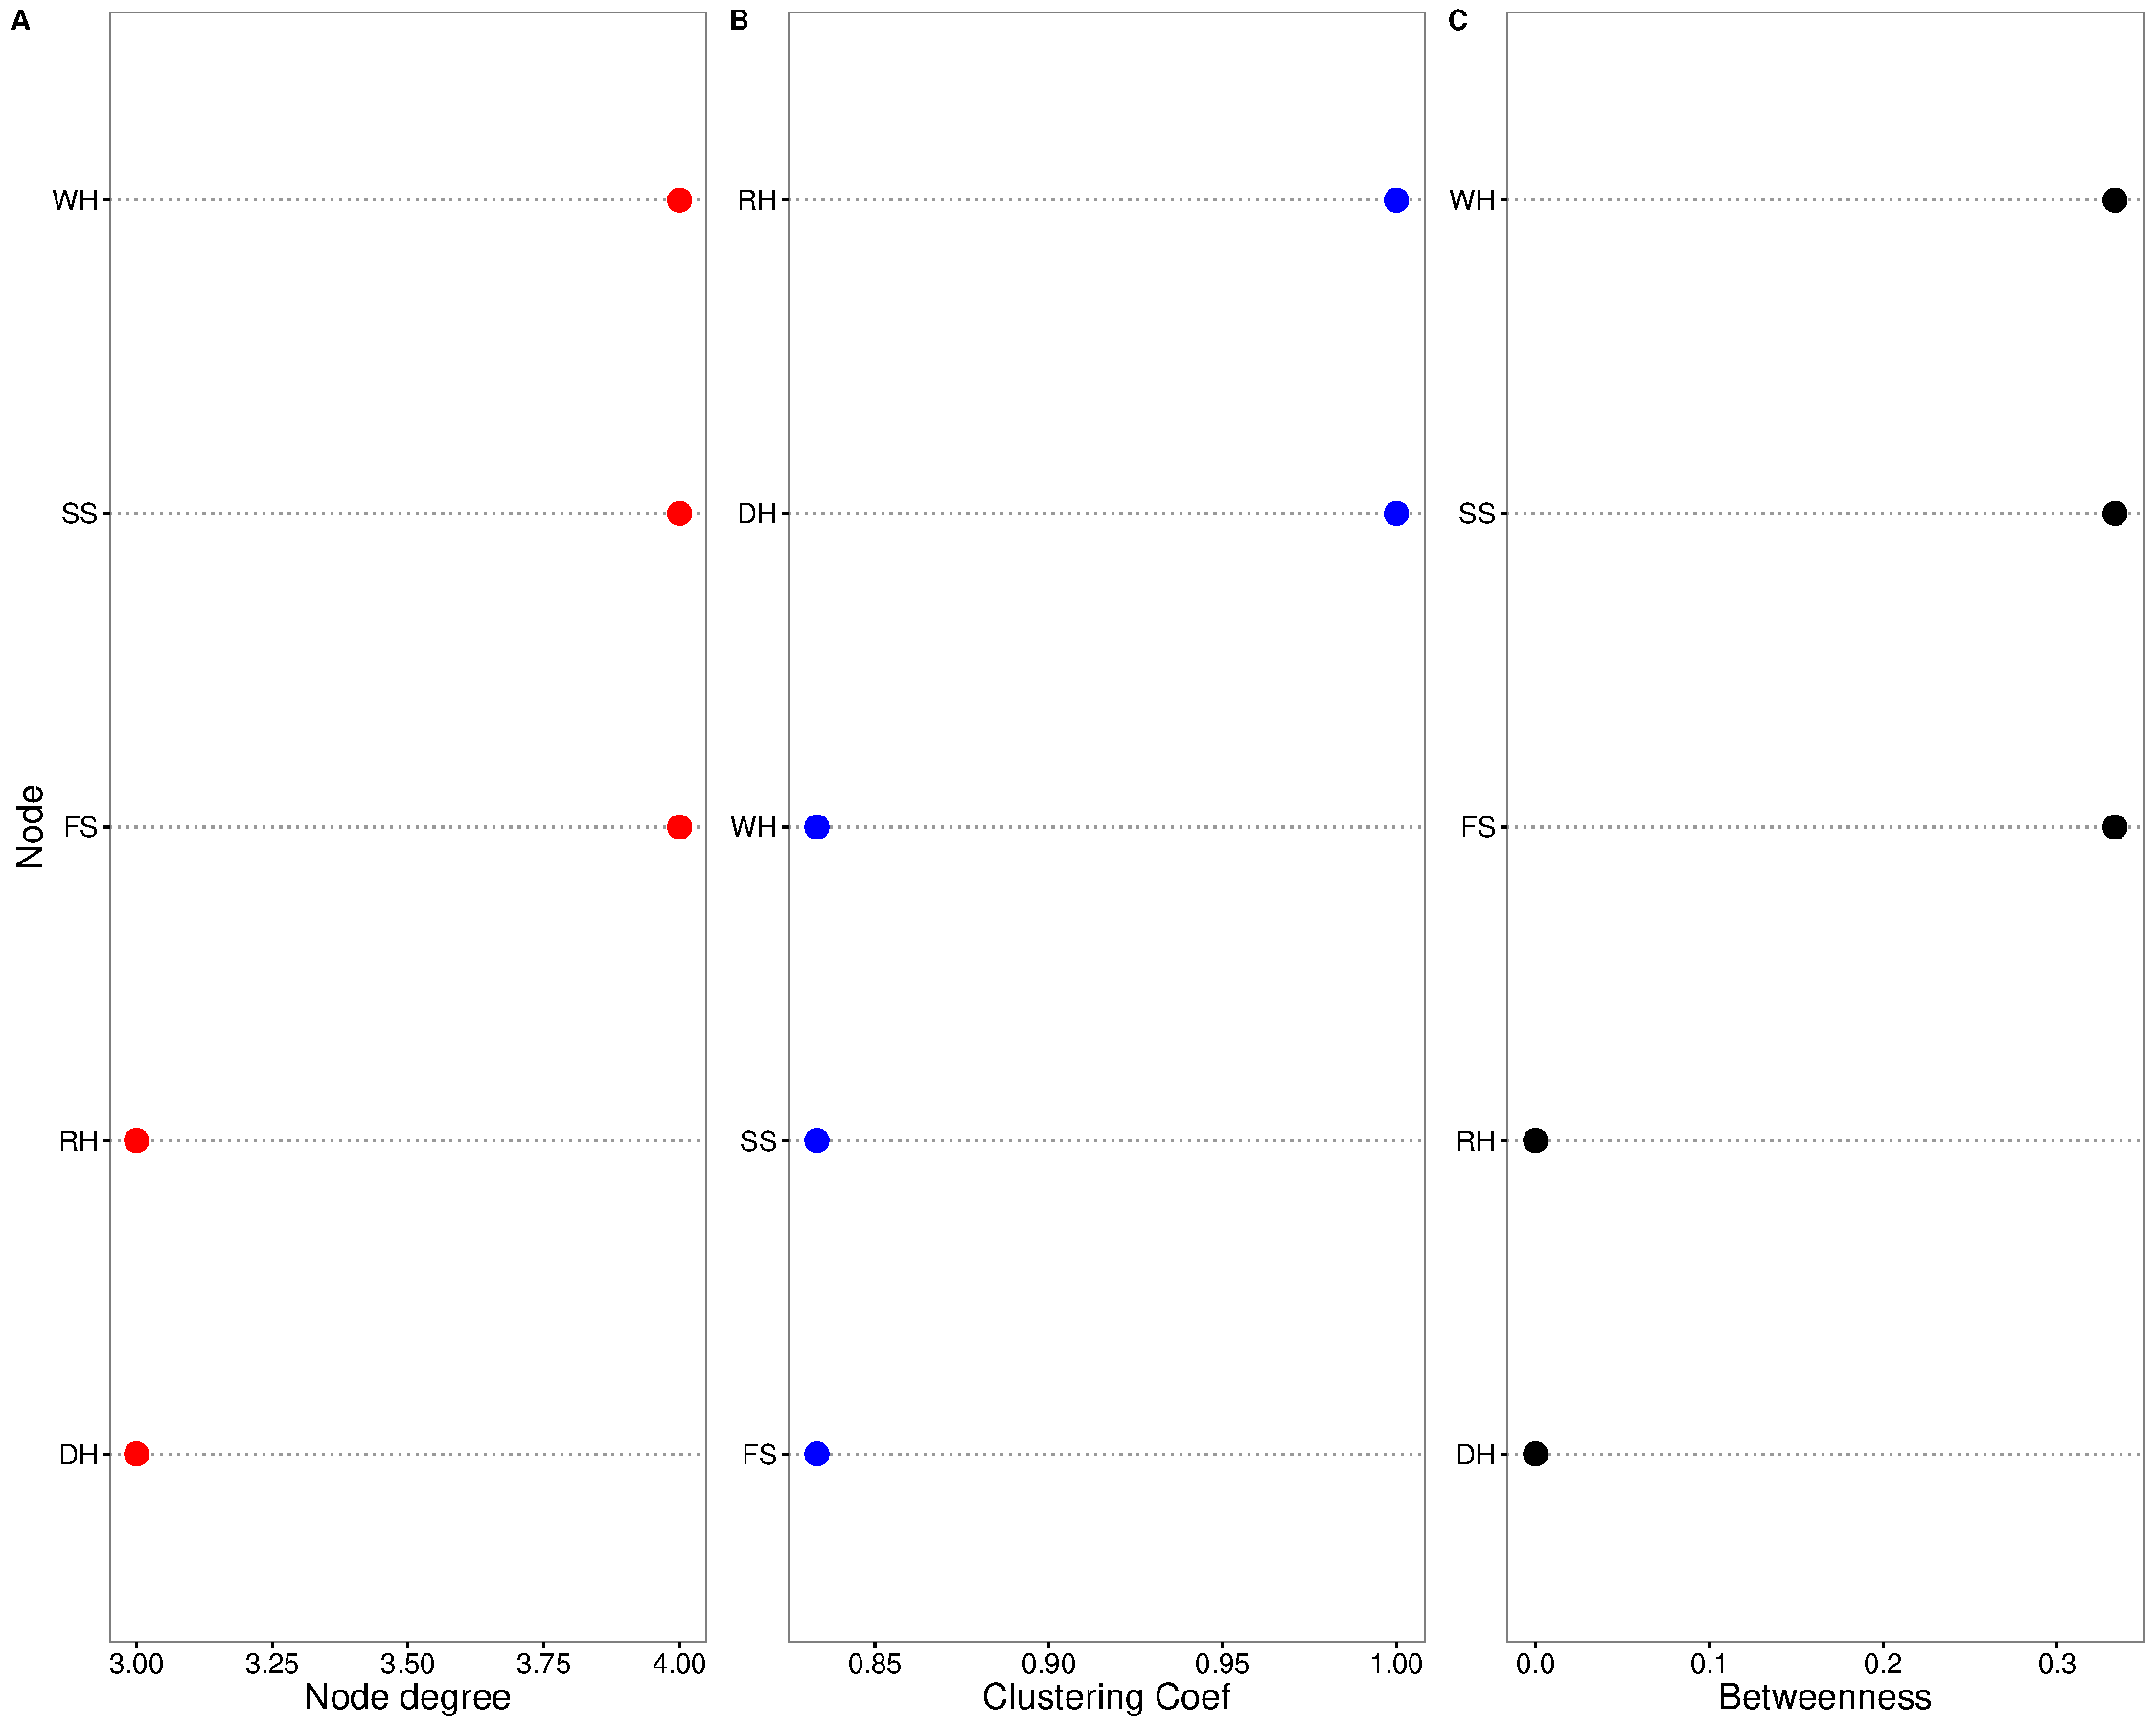
\includegraphics[width = 1\textwidth]{figures/yield_dif_nodepropOdisha.pdf}
        \caption[Three centrality measures of the nodes in co-occurrence network of rice injuries in dry season at Odisha, India.]{Three centrality measures of the nodes in co-occurrence network of rice injuries in dry season at Odisha, India. A: node degree, B:clustering coefficient, and C:Betweenness.}
        \label{fig:nodepropdifyield_OD}
    \end{subfigure}
    \caption{Differential network analysis of survey data in different yield levels at Odisha, India.}
    \label{fig:difyield_OD}
\end{figure}
 
 \begin{figure}
    \centering
    \begin{subfigure}[b]{1\textwidth}
        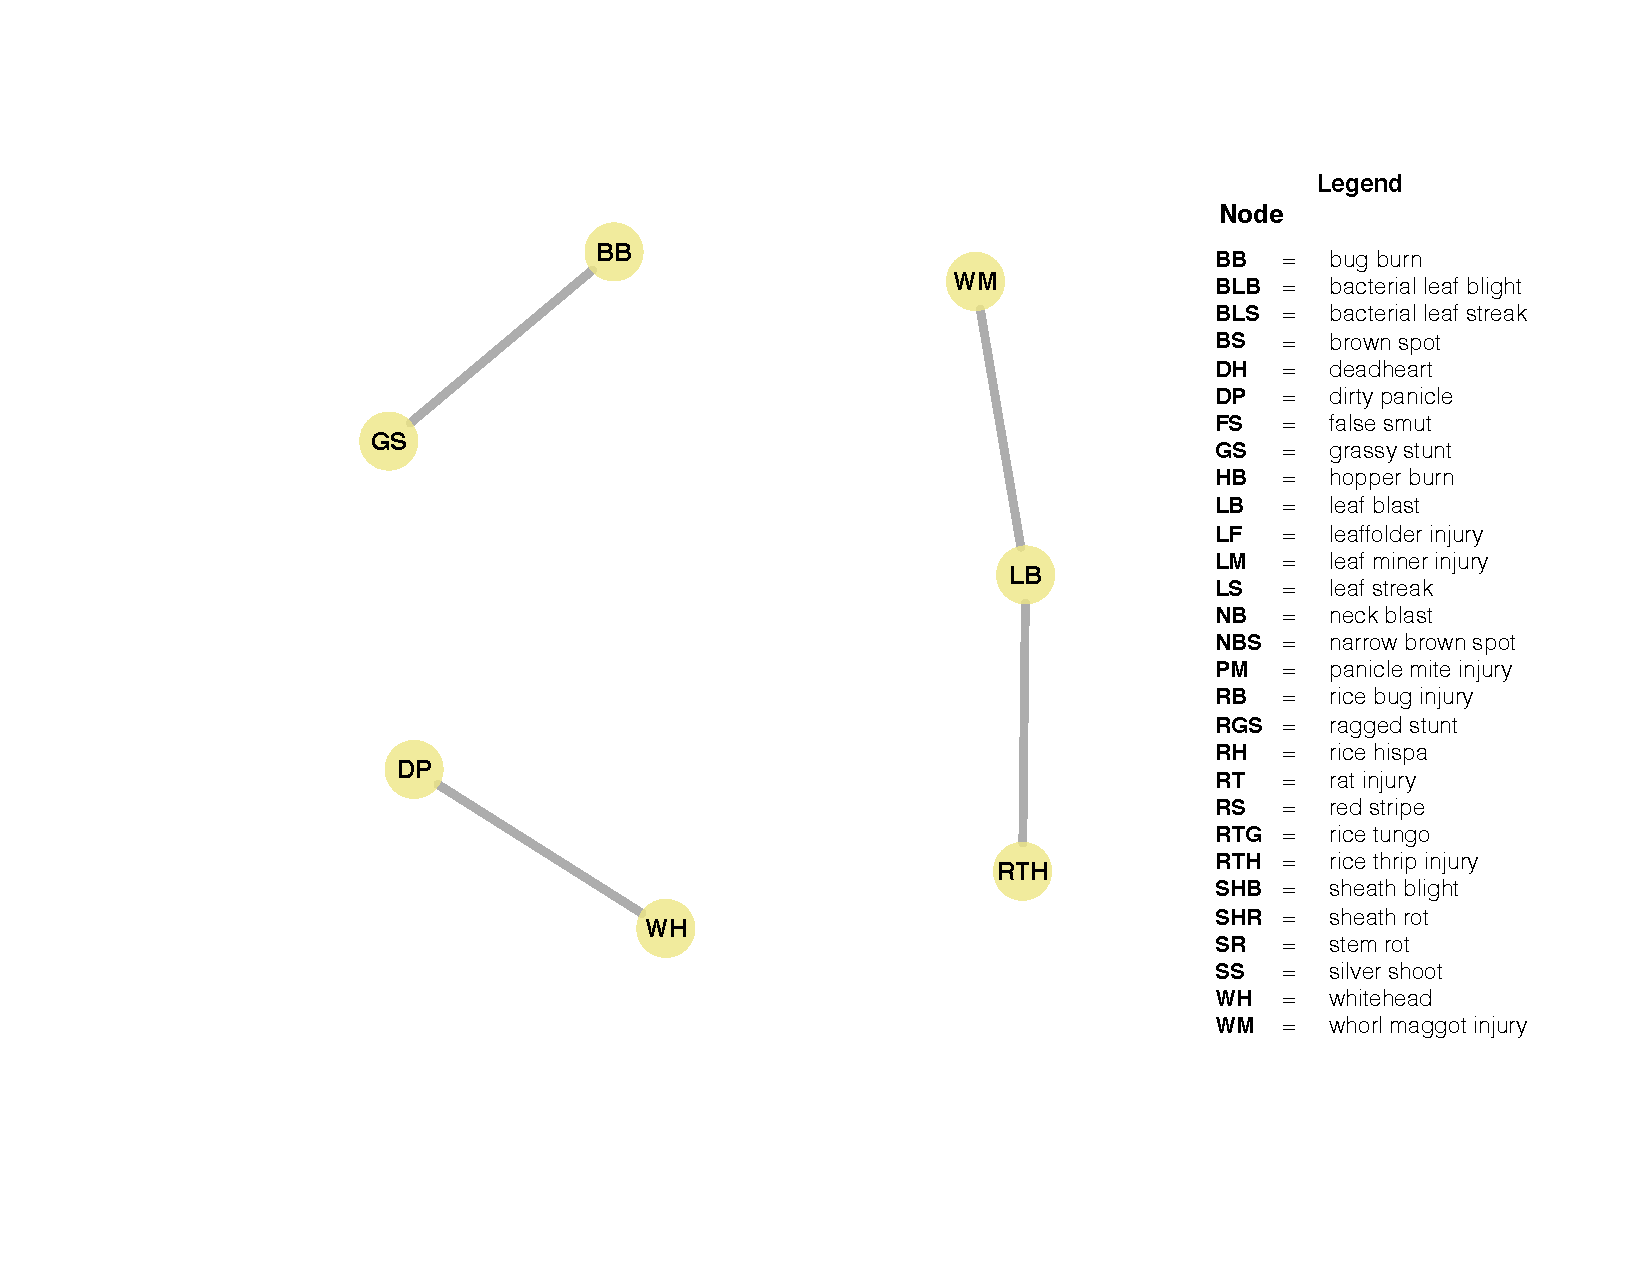
\includegraphics[width = 1\textwidth]{figures/difyieldRR.pdf}
        \caption[Differential co-occurrence network of rice injuries in different yield levels at Red River Delta, Vietnam. ]{Differential co-occurrence network of rice injuries in different yield levels at Red River Delta, Vietnam. The layout of the network graph is based on the Fruchterman-Reingold algorithm, which places nodes with stronger or more connections closer to each other.}
        \label{fig:difyieldnetwork_RR}
    \end{subfigure}
    \begin{subfigure}[b]{1\textwidth}
        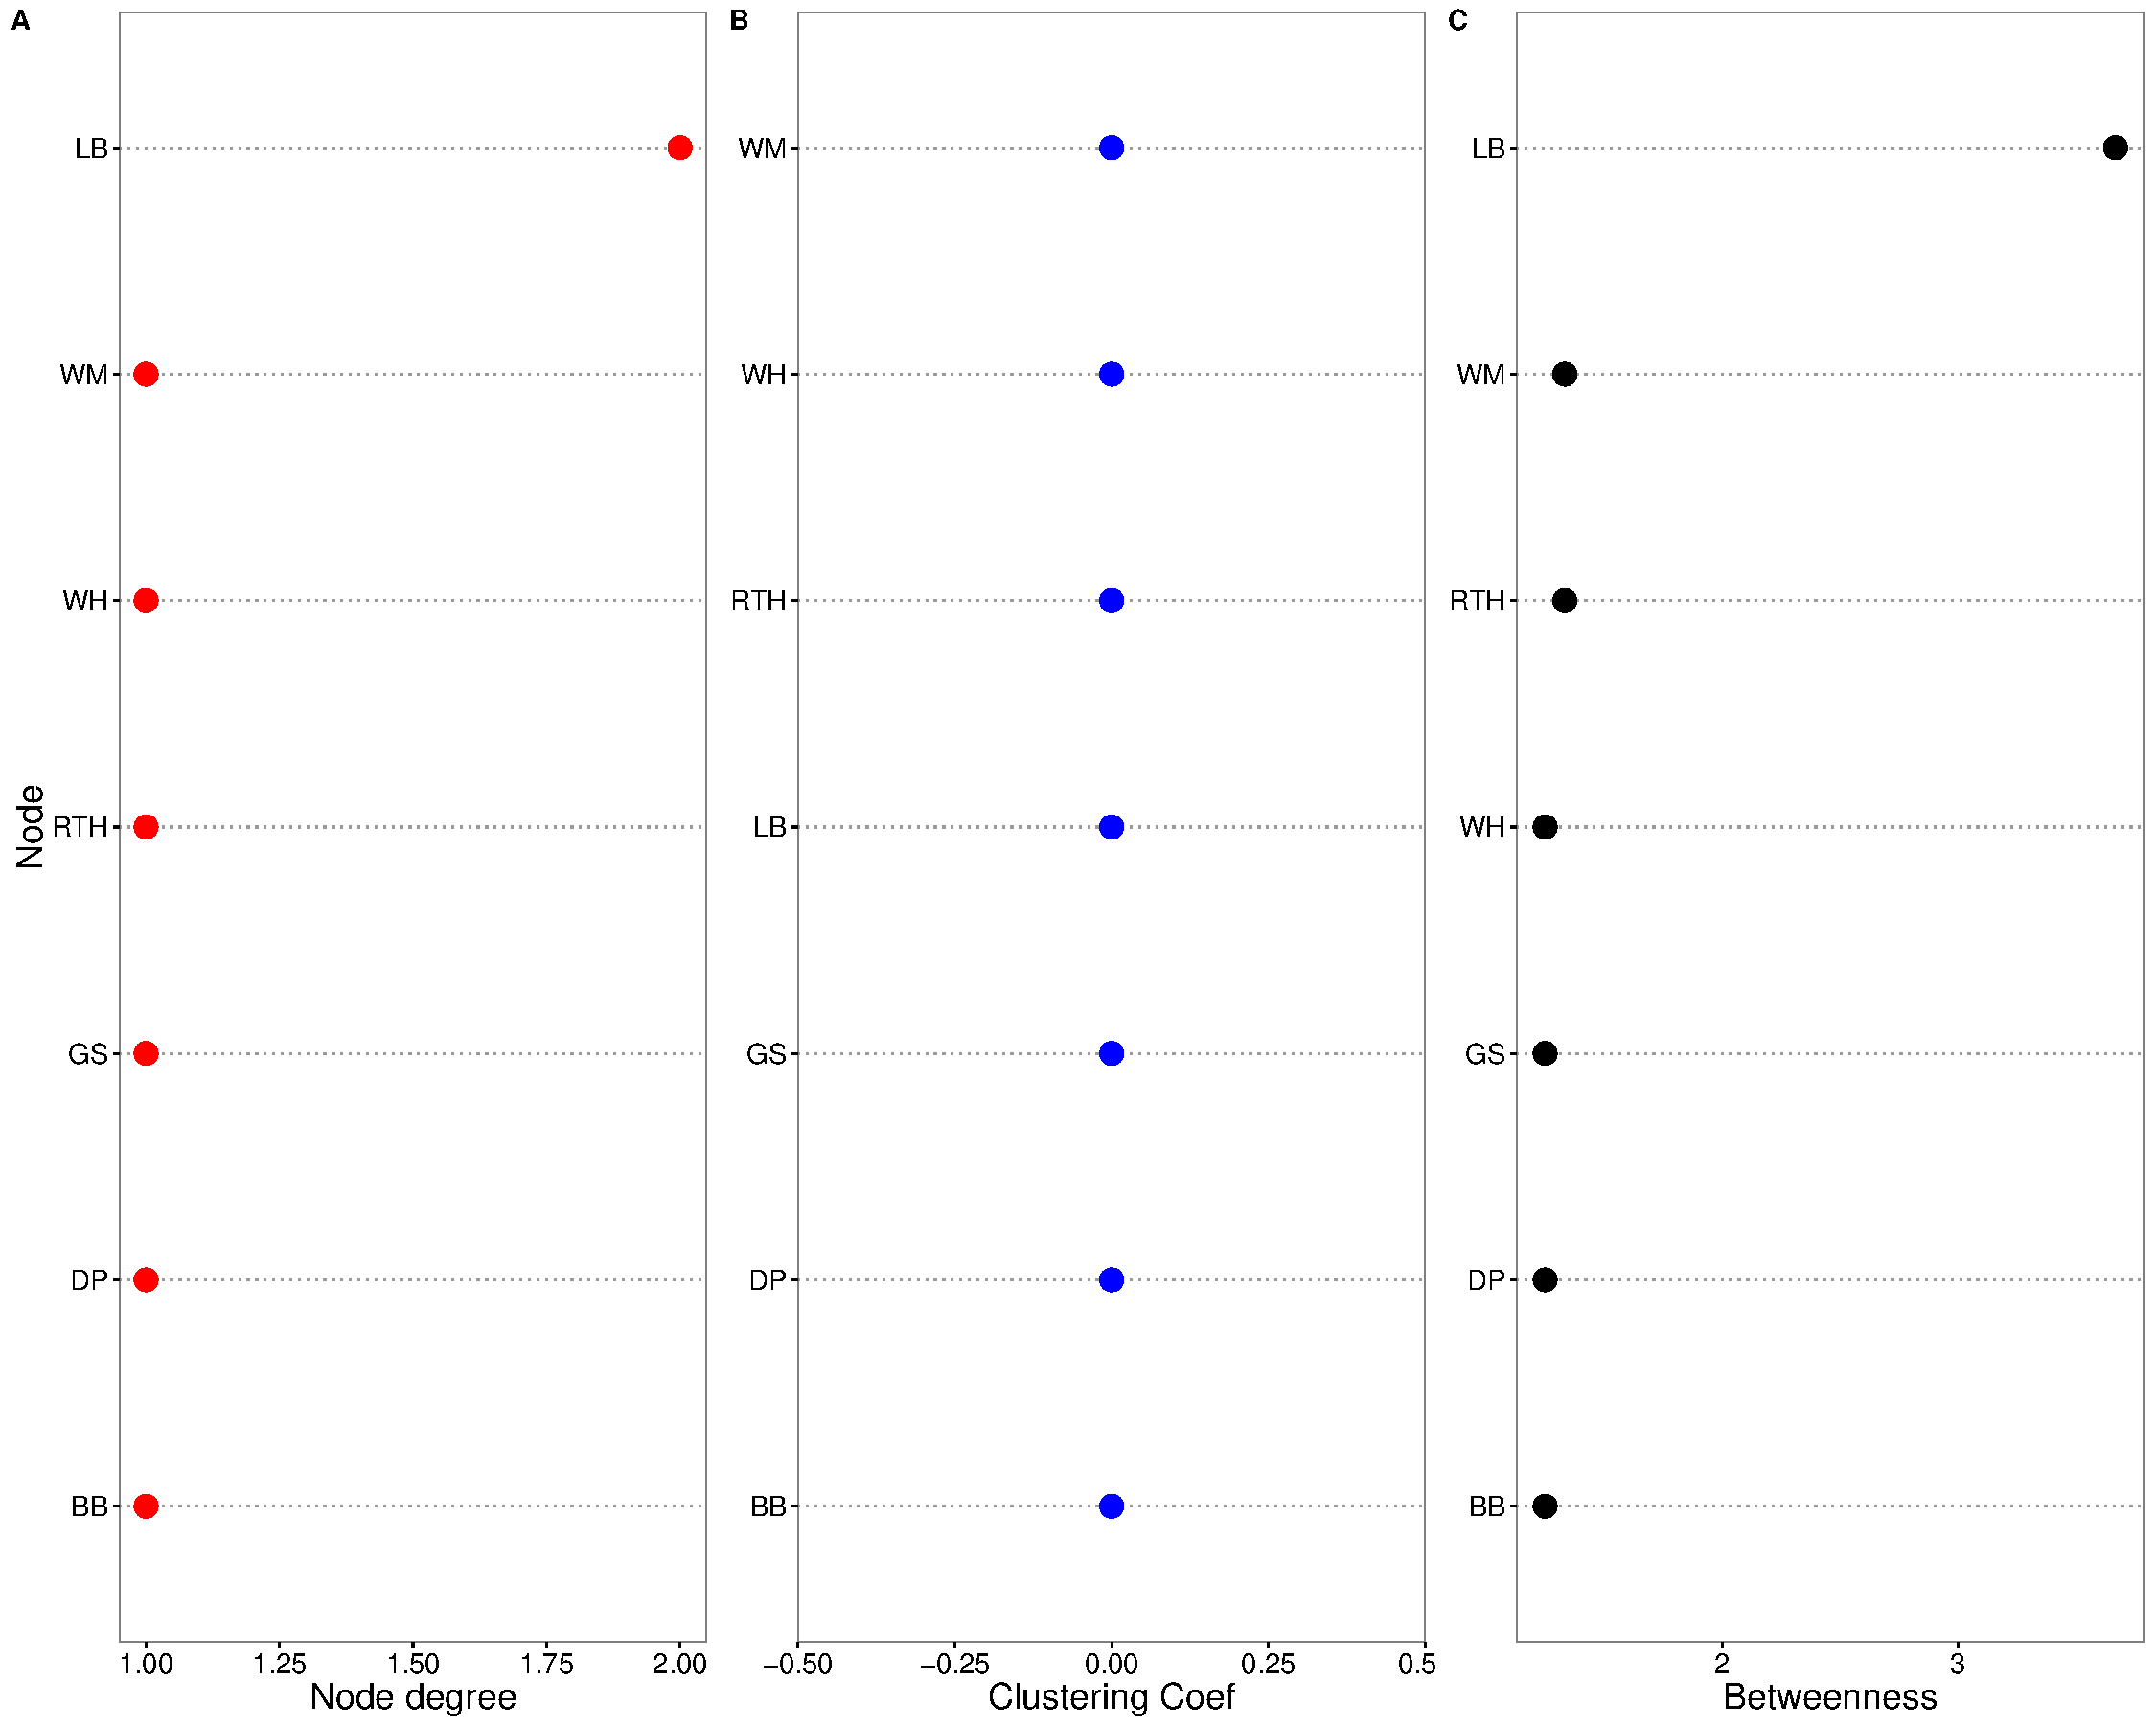
\includegraphics[width = 1\textwidth]{figures/yield_dif_nodepropRed_River_Delta.pdf}
        \caption[Three centrality measures of the nodes in differential co-occurrence network of rice injuries in different yield levels at Red River Delta, Vietnam]{Three centrality measures of the nodes in differential co-occurrence network of rice injuries in different yield levels at Red River Delta, Vietnam. A: node degree, B:clustering coefficient, and C:Betweenness.}
        \label{fig:nodepropdifyield_RR}
    \end{subfigure}
    \caption{Differential network analysis of survey data in different yield levels at Red River Delta, Vietnam}
    \label{fig:difyield_RR}
\end{figure}
 
 \begin{figure}
    \centering
    \begin{subfigure}[b]{1\textwidth}
        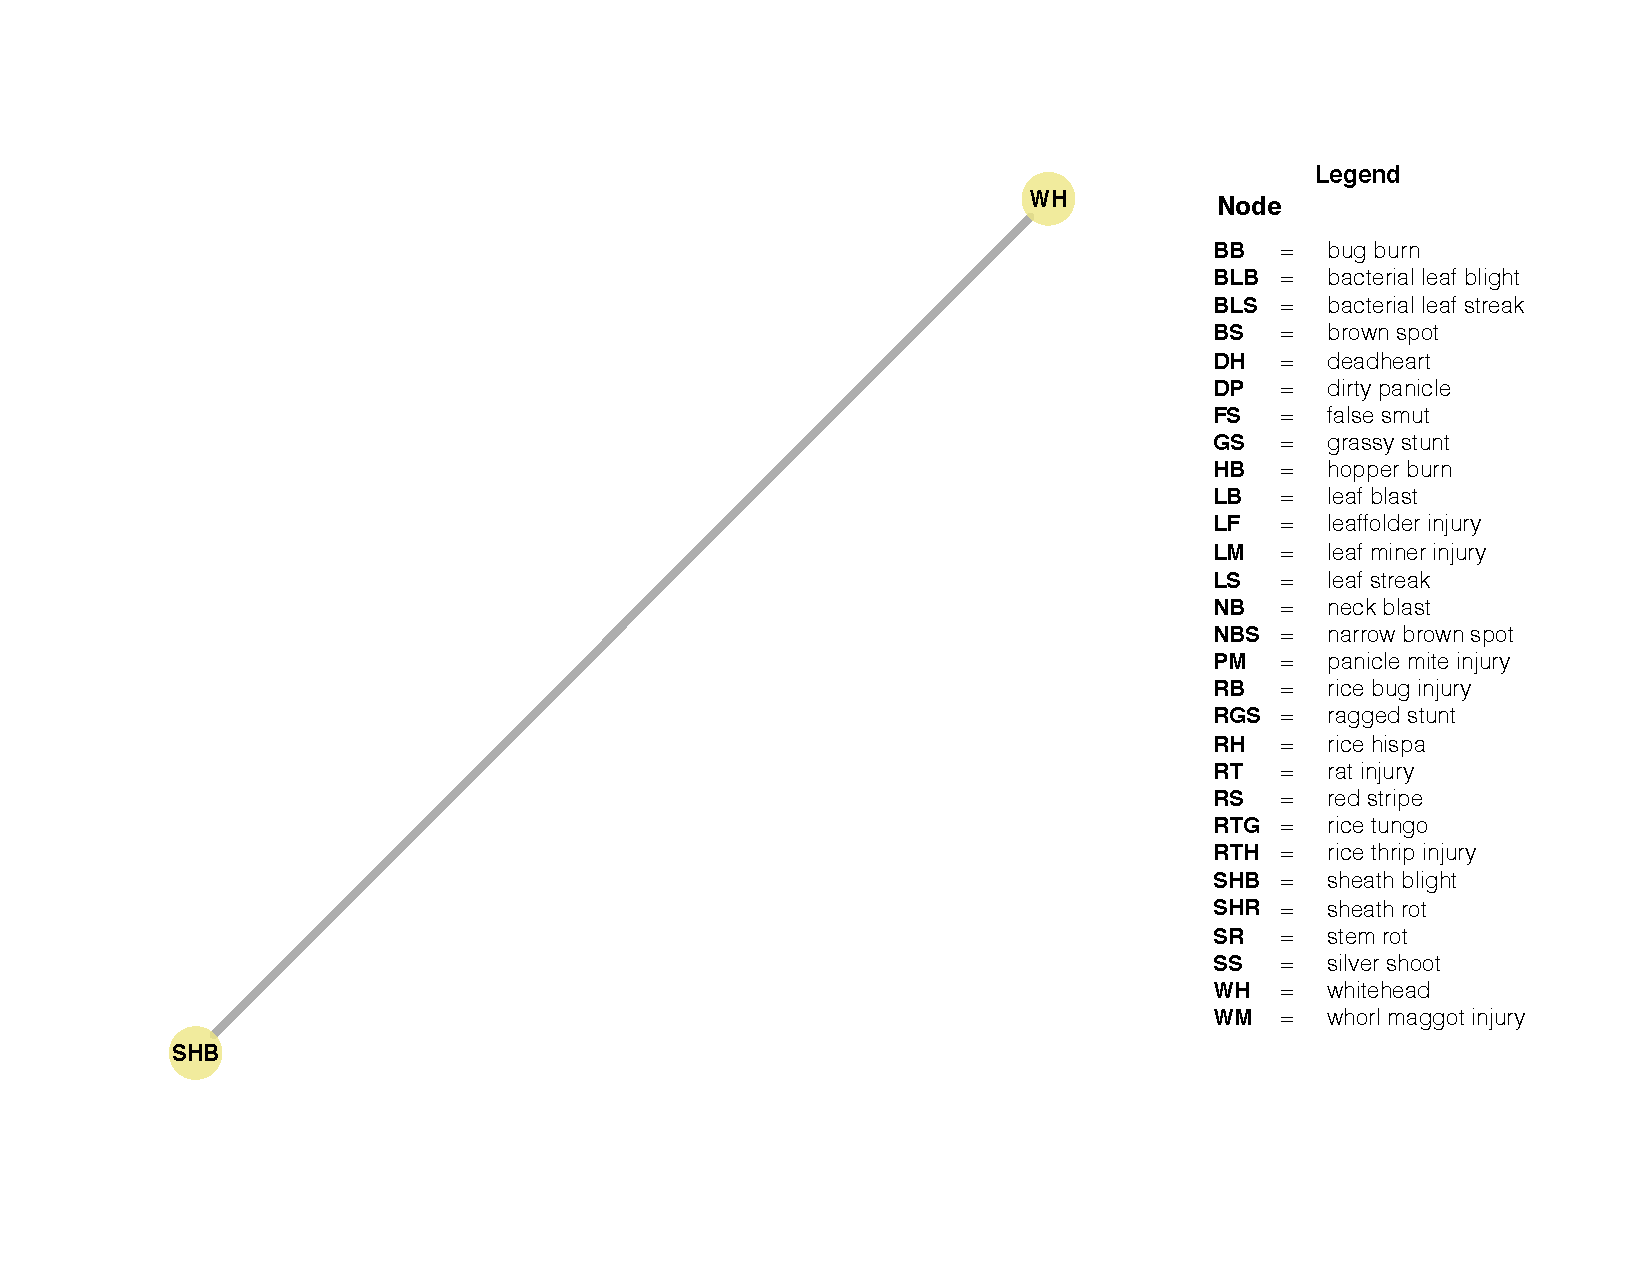
\includegraphics[width = 1\textwidth]{figures/difyieldTM.pdf}
        \caption[Differential co-occurrence network of rice injuries in different yield levels at Tamil Nadu, India.]{Differential co-occurrence network of rice injuries in different yield levels at Tamil Nadu, India. The layout of the network graph is based on the Fruchterman-Reingold algorithm, which places nodes with stronger or more connections closer to each other.}
        \label{fig:difyieldnetwork_TM}
    \end{subfigure}
    \begin{subfigure}[b]{1\textwidth}
        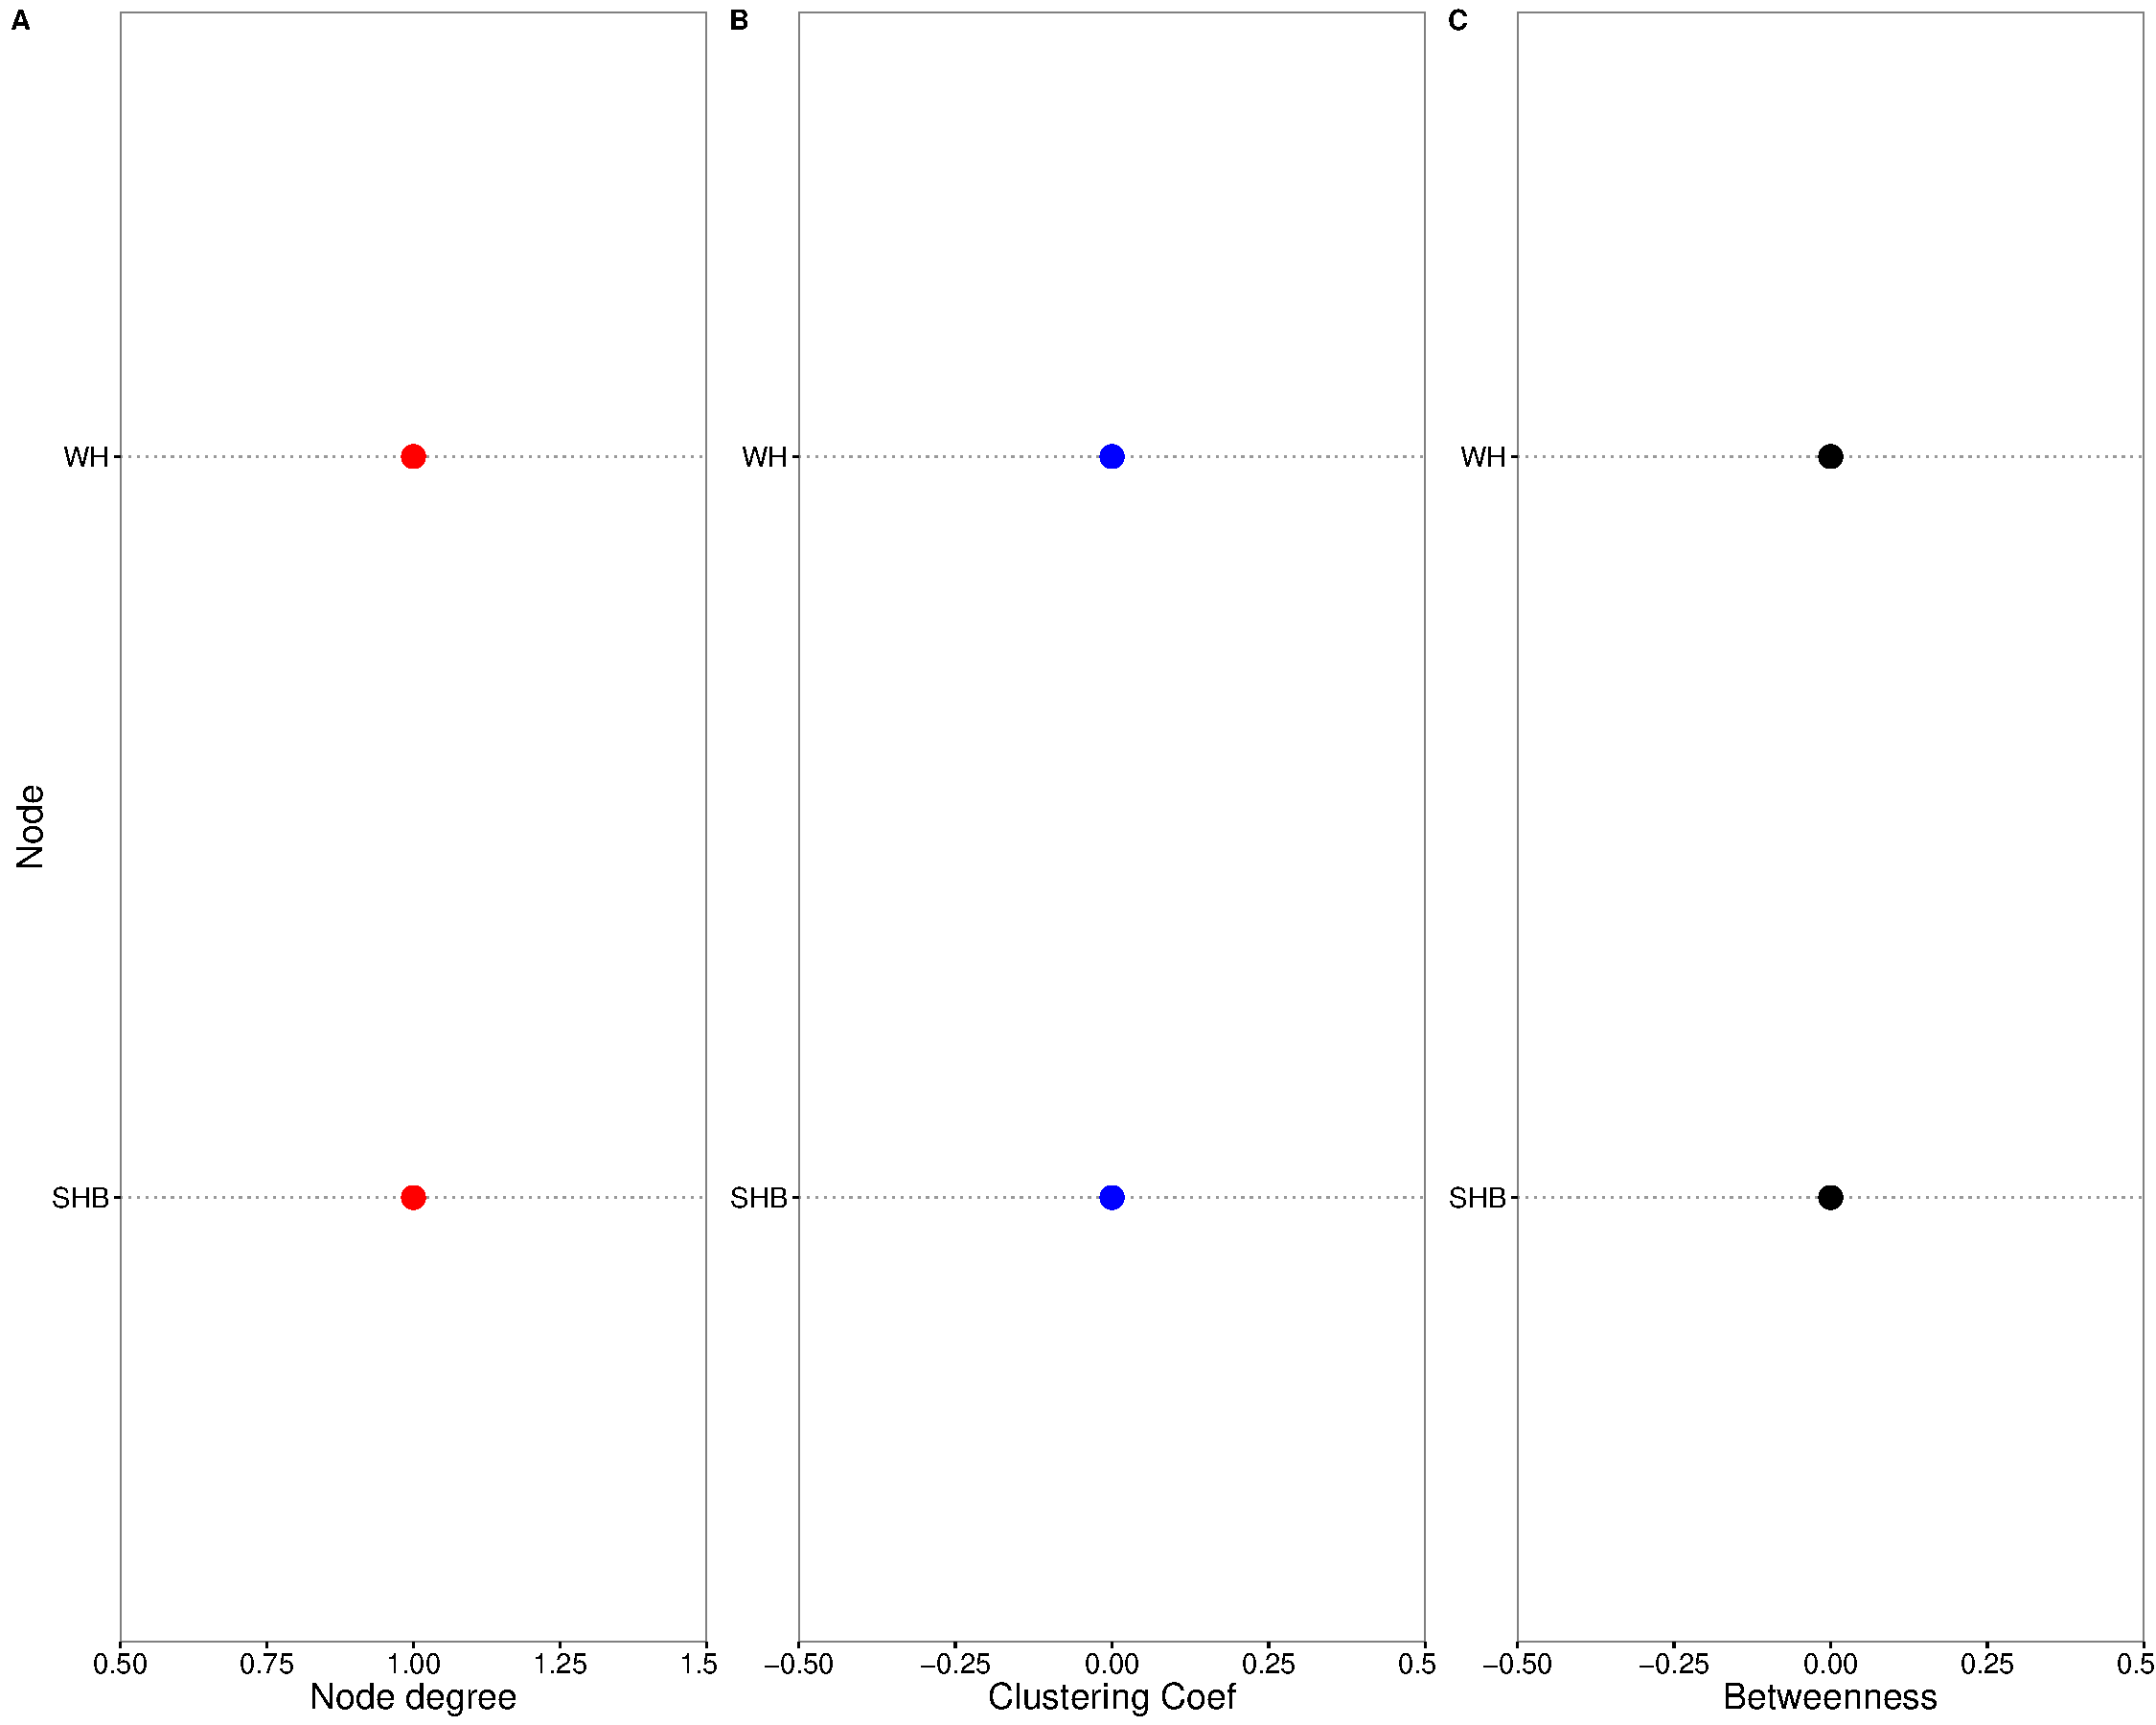
\includegraphics[width = 1\textwidth]{figures/yield_dif_nodepropTamil_Nadu.pdf}
        \caption{Three centrality measures of the nodes in co-occurrence network of rice injuries in dry season at Central Plain. A: node degree, B:clustering coefficient, and C:Betweenness.}
        \label{fig:nodepropdifyield_TM}
    \end{subfigure}
    \caption{Differential network analysis of survey data in different yield levels at Tamil Nadu, India.}
    \label{fig:yielddif_TM}
\end{figure}
 
  
 \begin{figure}
    \centering
    \begin{subfigure}[b]{1\textwidth}
        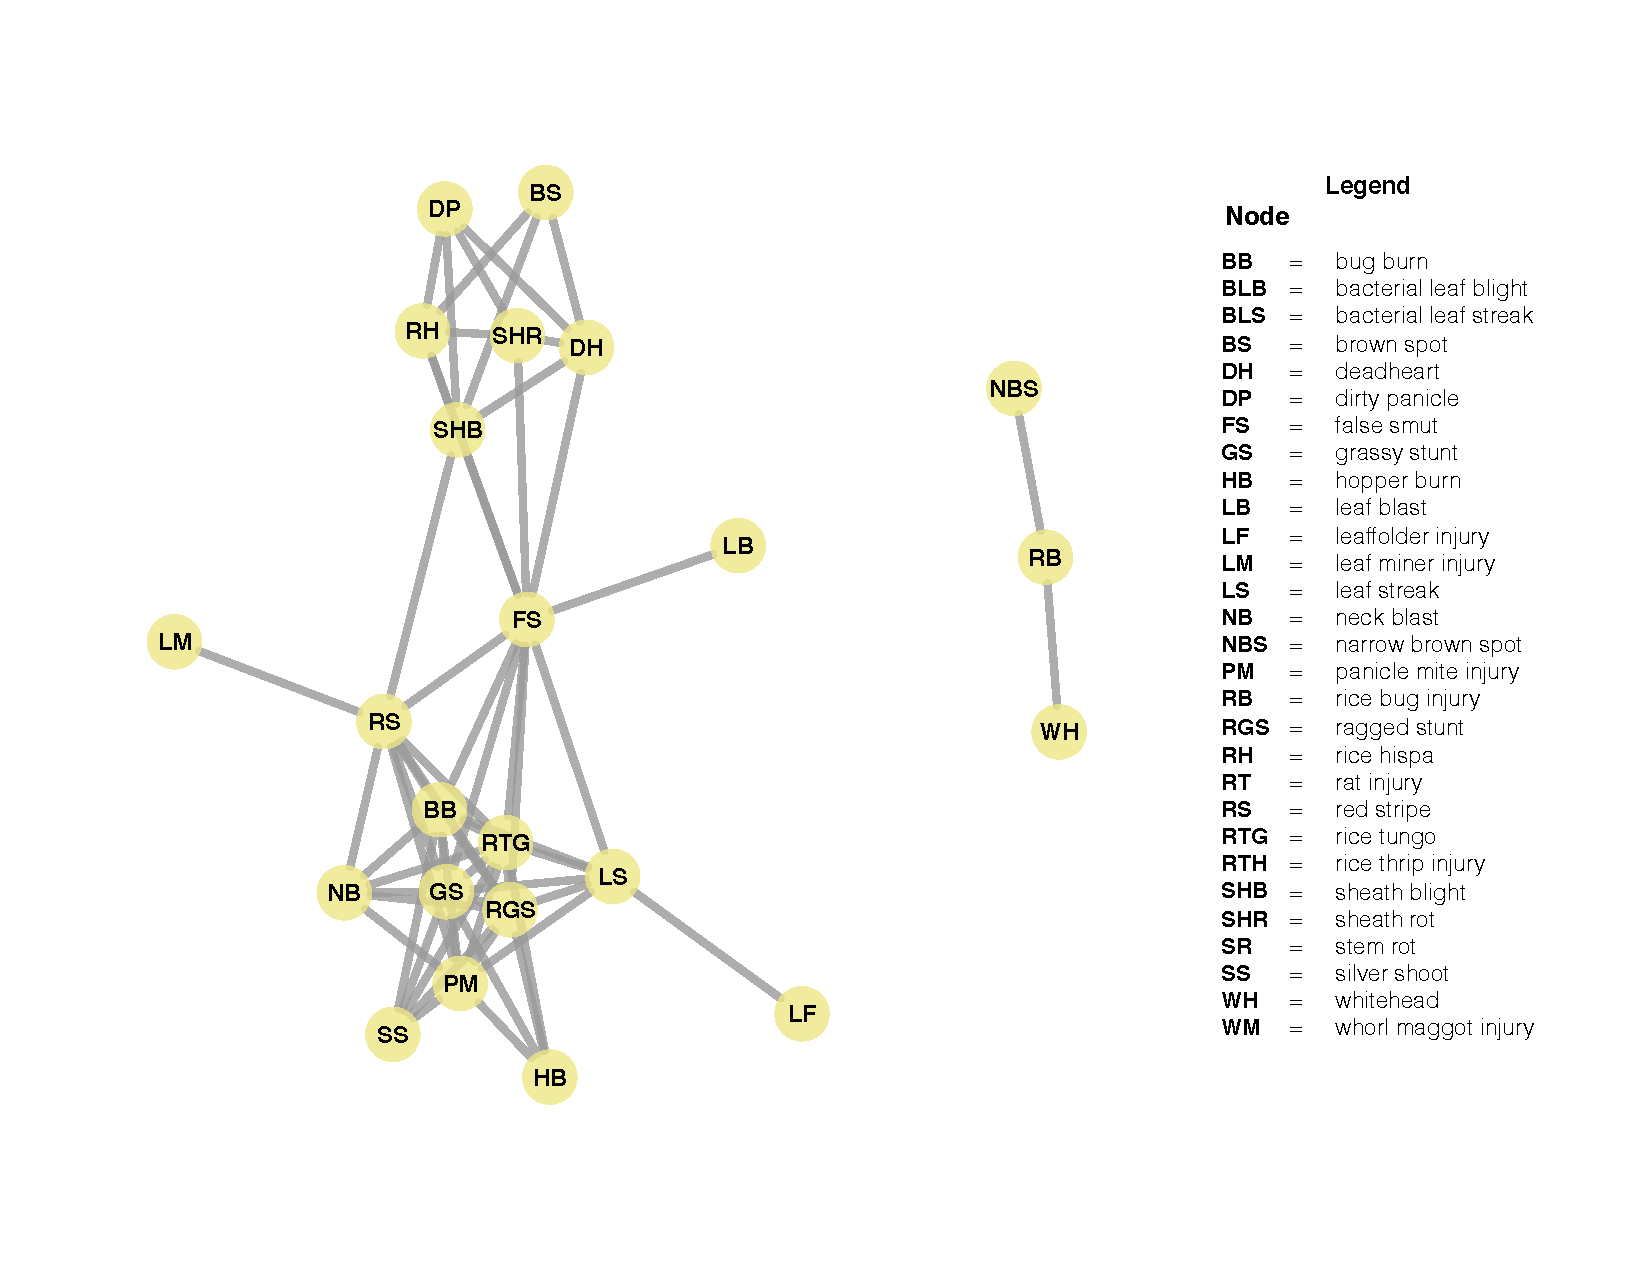
\includegraphics[width = 1\textwidth]{figures/difyieldWJ.pdf}
        \caption[Differential co-occurrence network of rice injuries in different yield levels at West Java, Indonesia.]{Differential co-occurrence network of rice injuries in different yield levels at West Java, Indonesia. The layout of the network graph is based on the Fruchterman-Reingold algorithm, which places nodes with stronger or more connections closer to each other.}
        \label{fig:difyieldnetwork_WJ}
    \end{subfigure}
    \begin{subfigure}[b]{1\textwidth}
        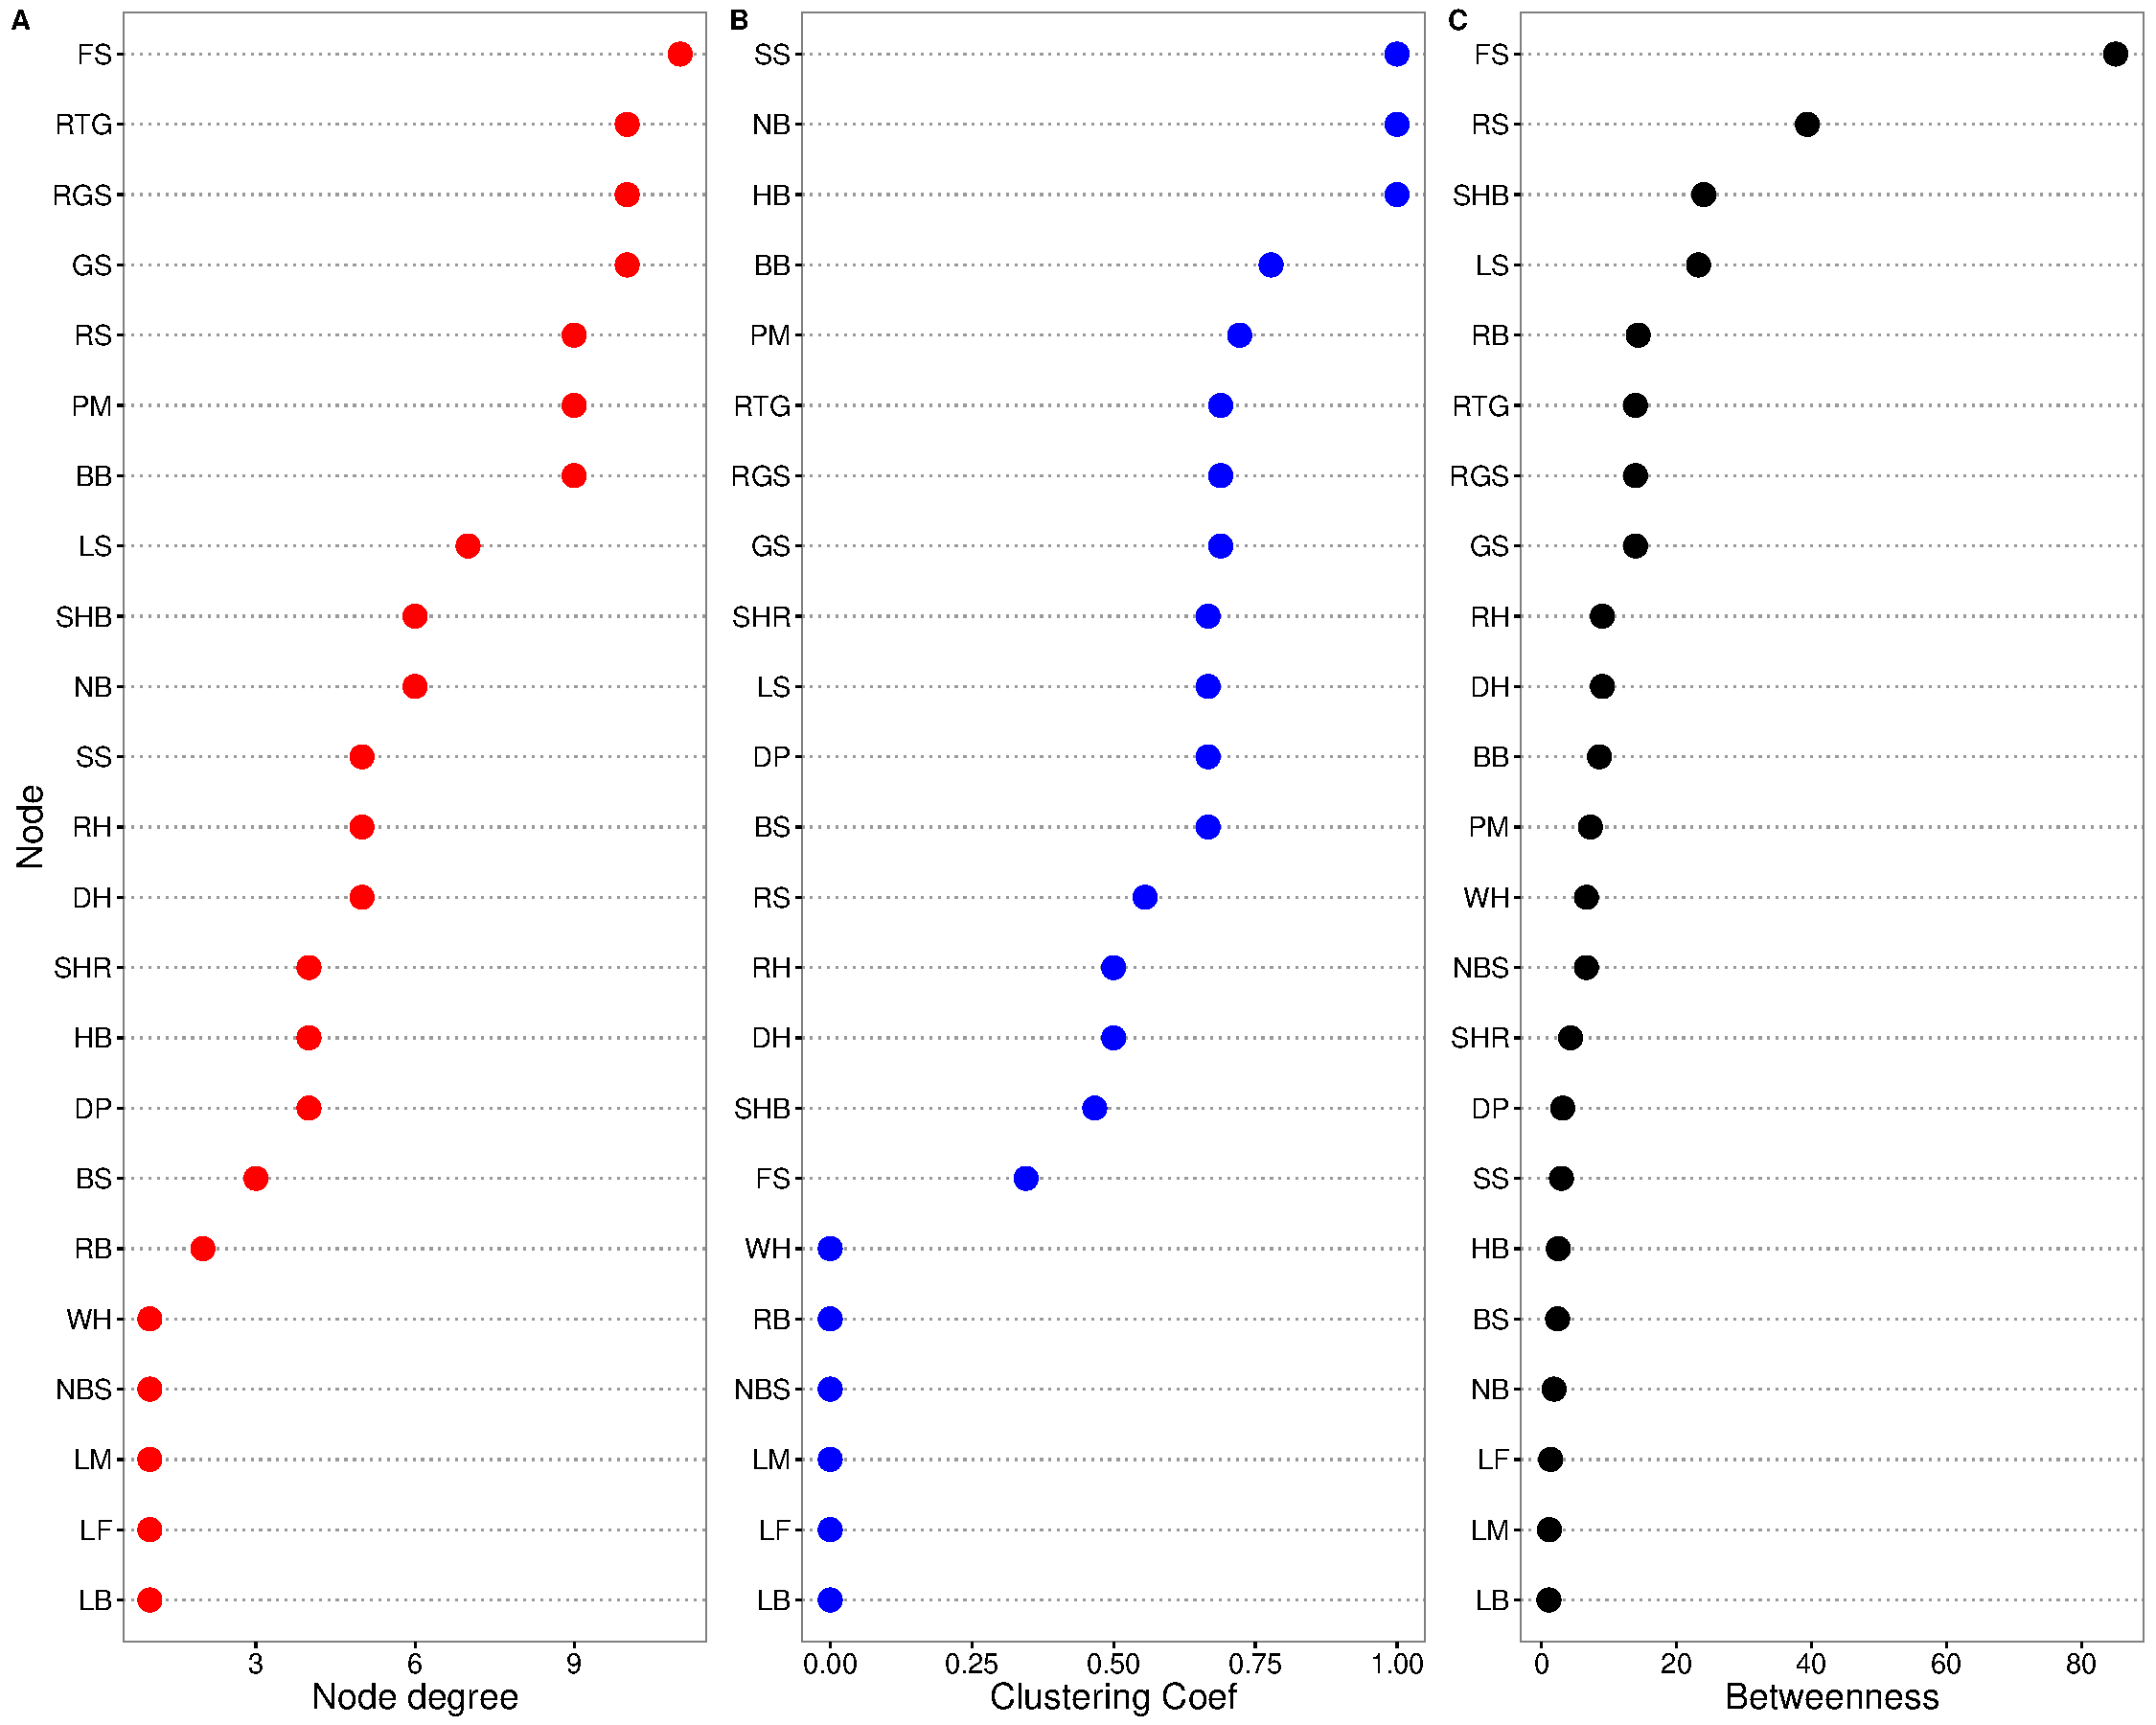
\includegraphics[width = 1\textwidth]{figures/yield_dif_nodepropWest_Java.pdf}
        \caption{Three centrality measures of the nodes in co-occurrence network of rice injuries in dry season at Central Plain. A: node degree, B:clustering coefficient, and C:Betweenness.}
        \label{fig:nodepropdifyield_WJ}
    \end{subfigure}
    \caption{Differential network analysis of survey data in different yield levels at West Java, Indonesia}
    \label{fig:yielddif_WJ}
\end{figure}


% ===
\begin{figure}[h]
    \centering
        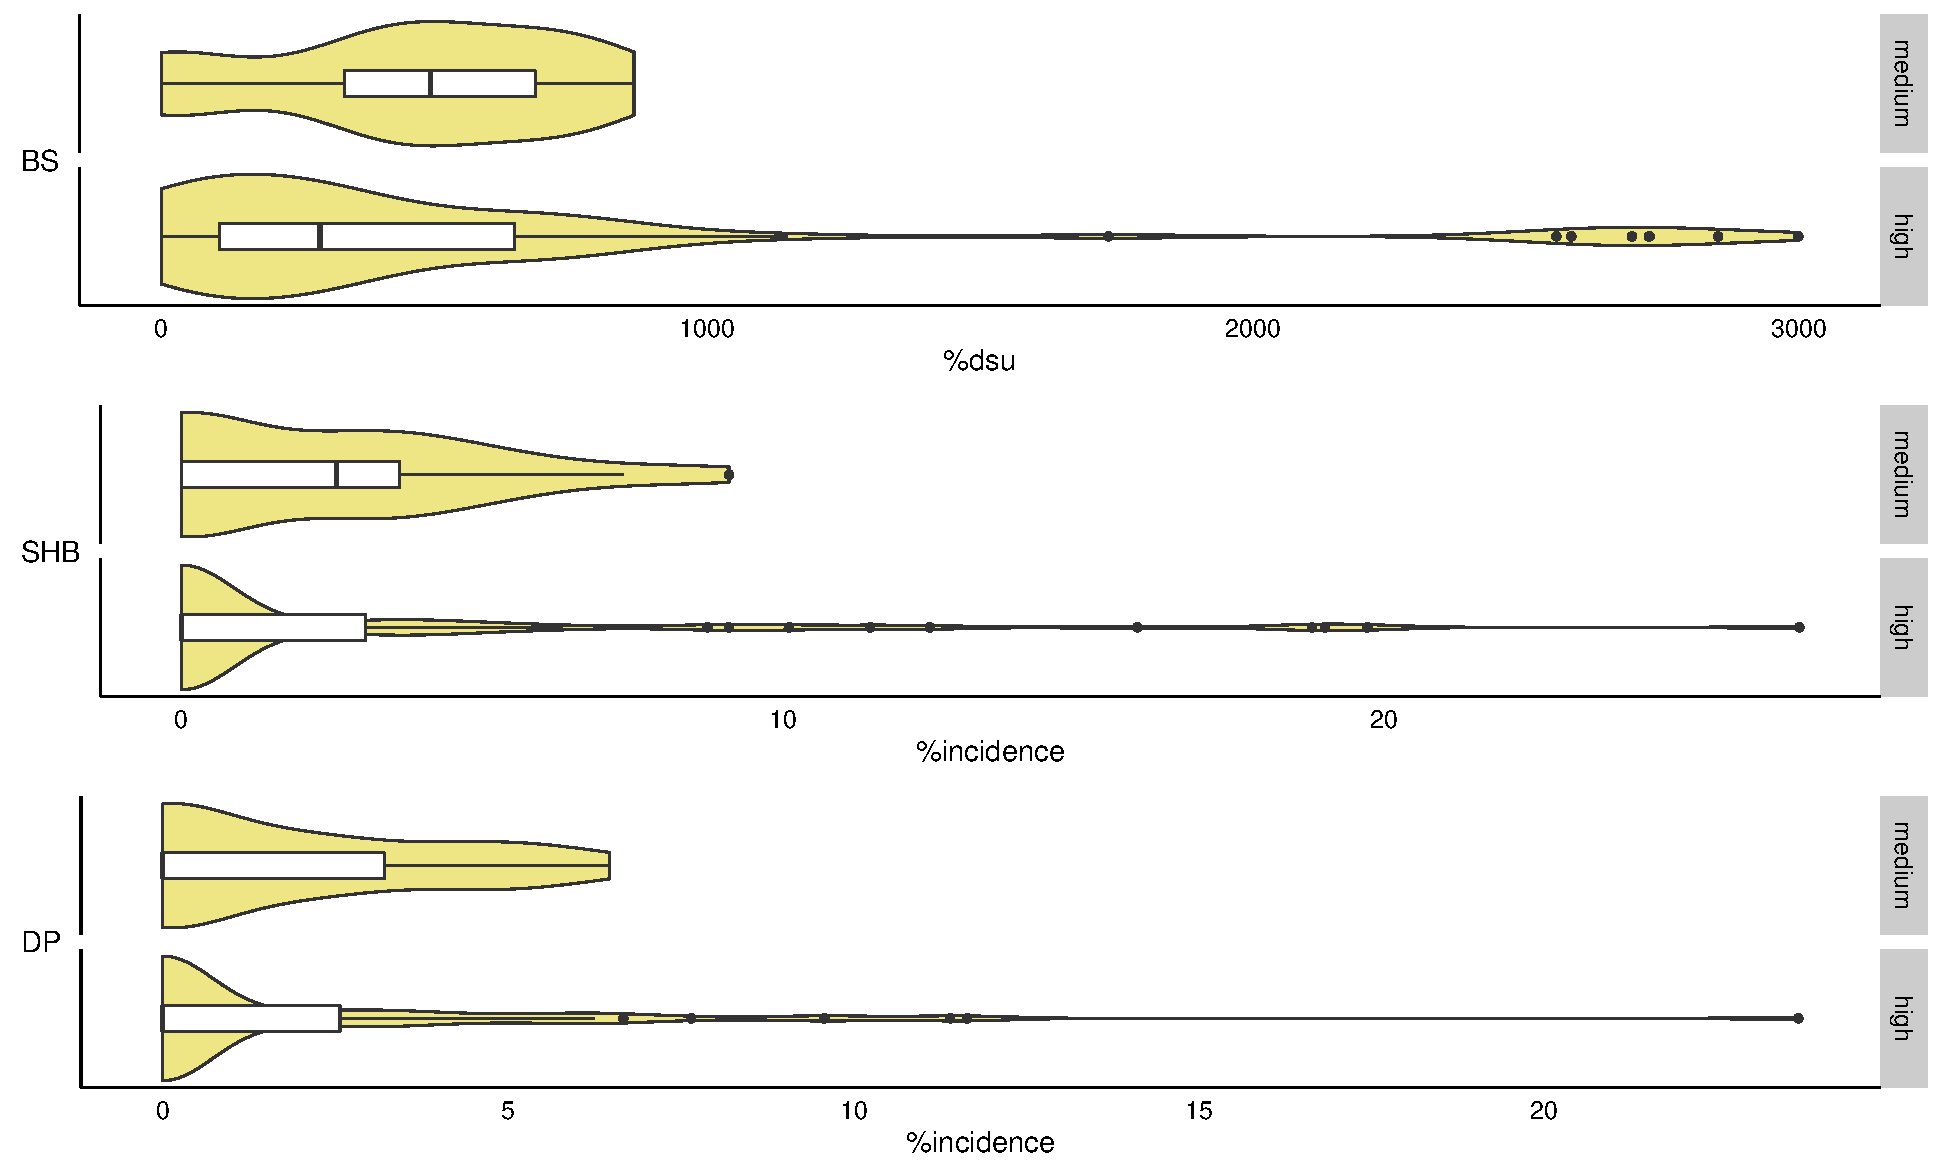
\includegraphics[width = 1\textwidth]{figures/CP_yield_box.pdf}
        \caption{.}
        \label{fig:yield.box_CP}
\end{figure}


\begin{figure}
        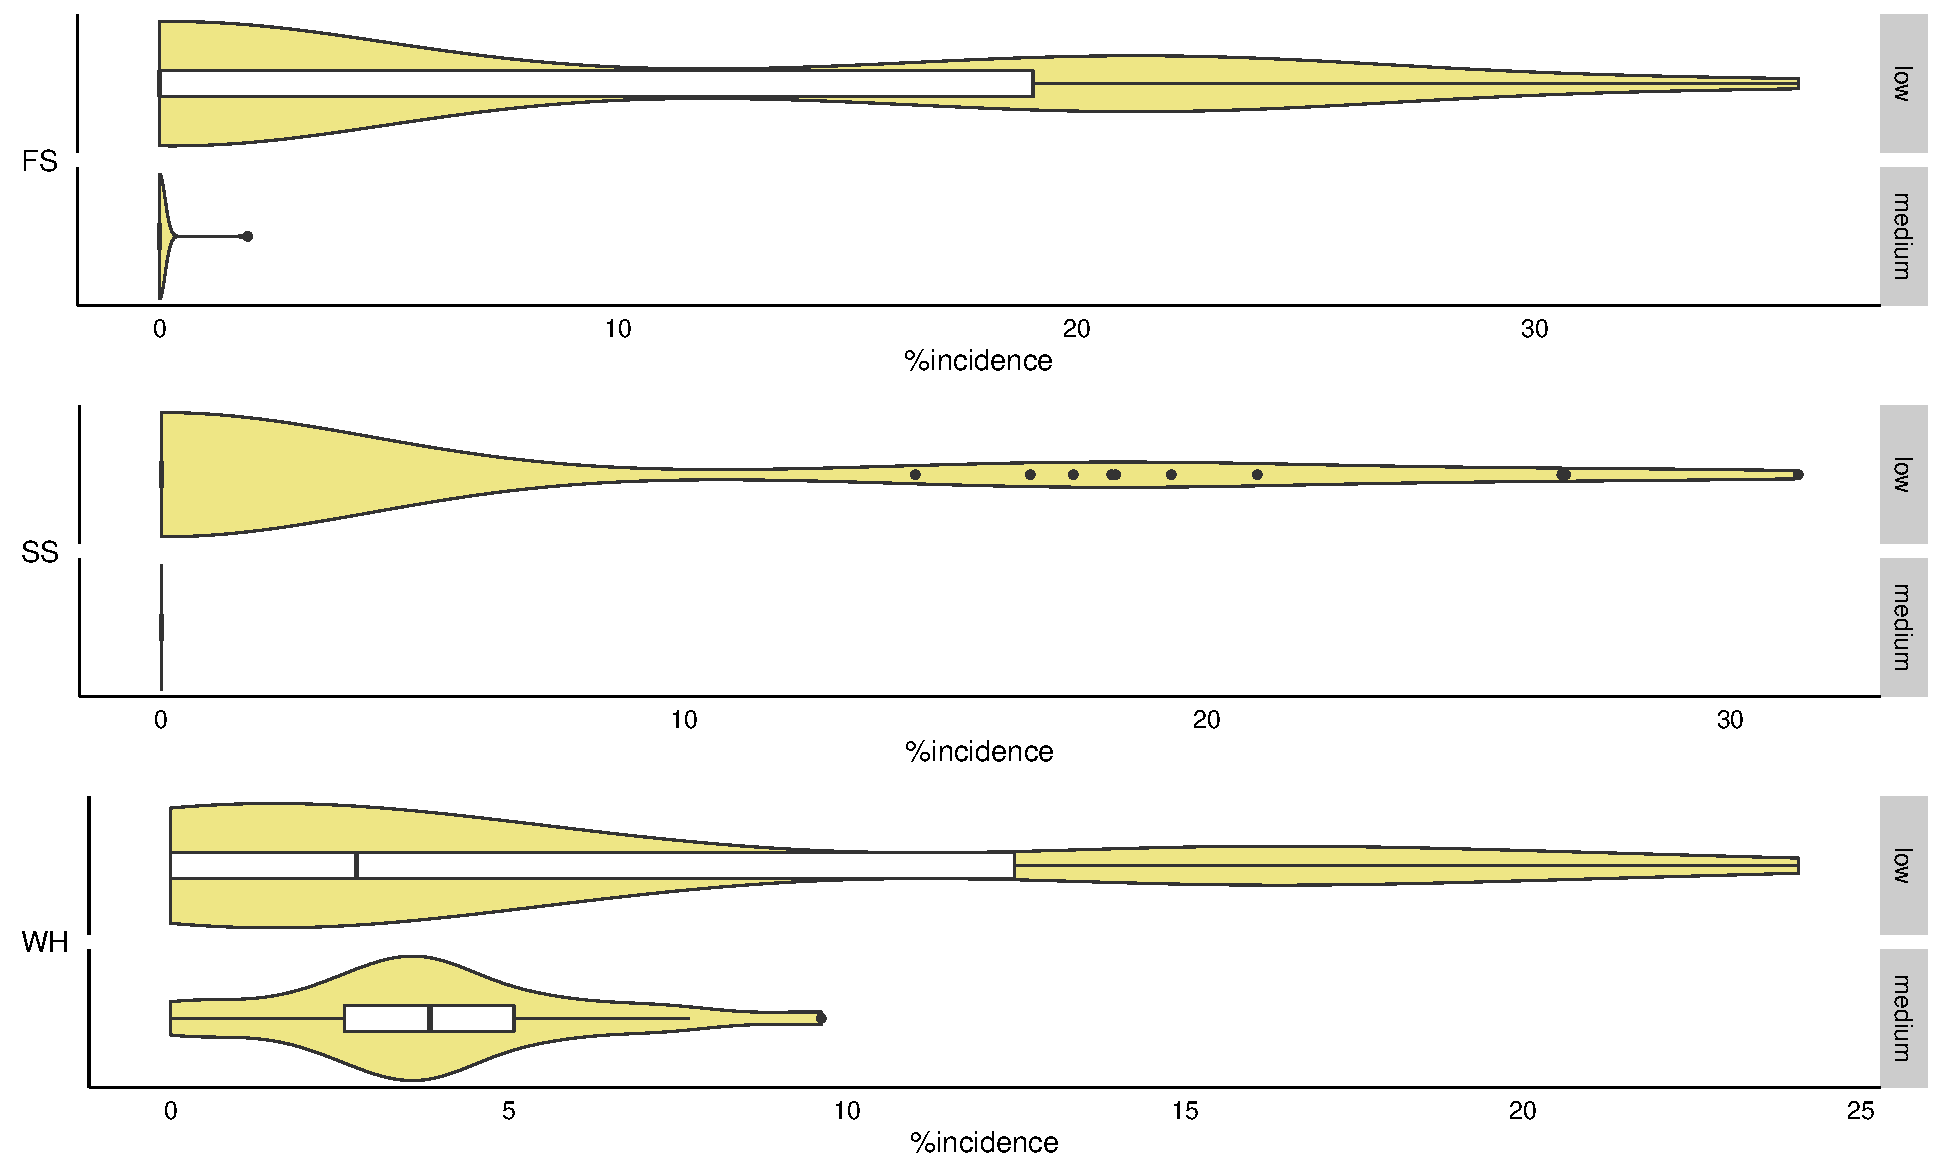
\includegraphics[width = 1\textwidth]{figures/OD_yield_box.pdf}
        \caption{.}
\label{fig:yield.box_OD}
\end{figure}

\begin{figure}
    \centering
        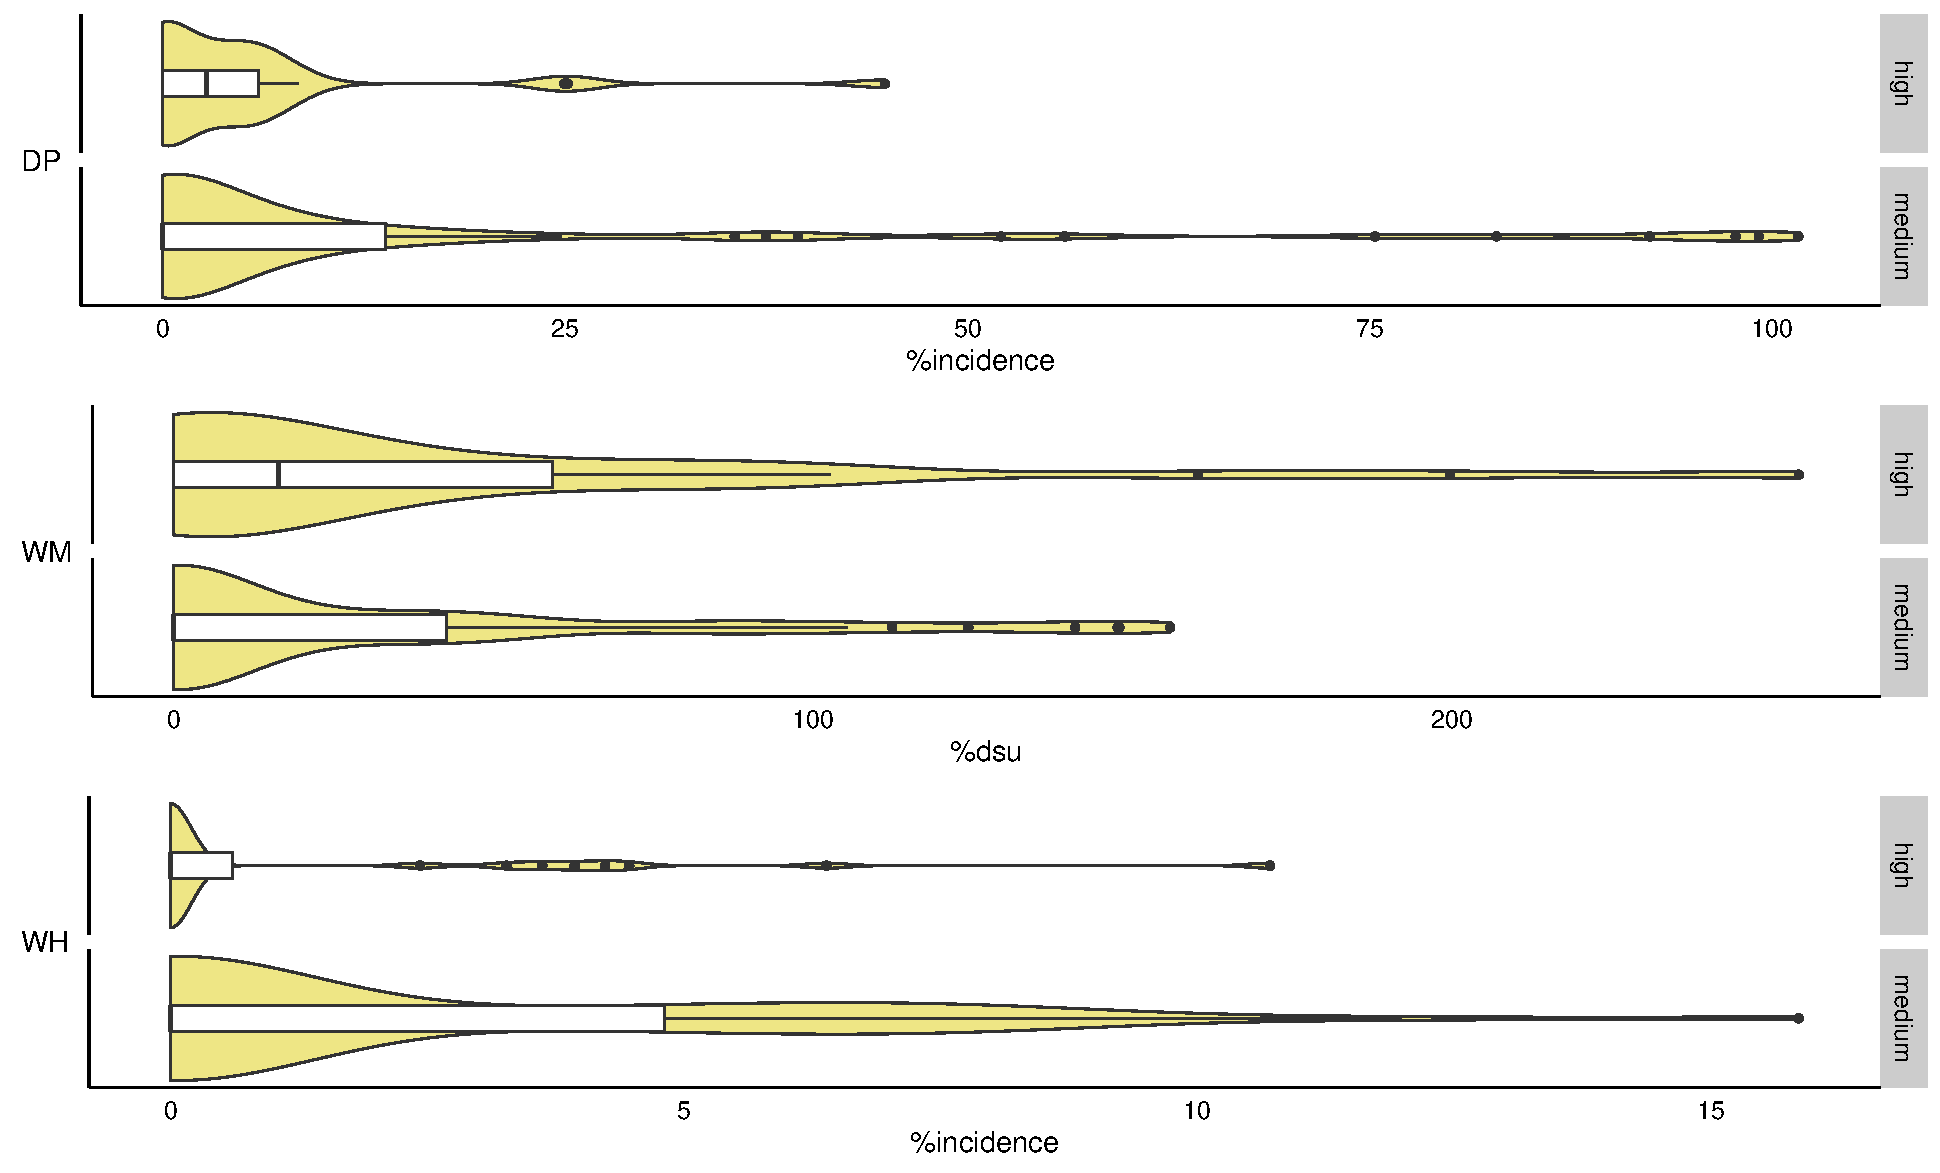
\includegraphics[width = 1\textwidth]{figures/RR_yield_box.pdf}
        \caption{.}
        \label{fig:yield.box_RR}
\end{figure}


\begin{figure}
        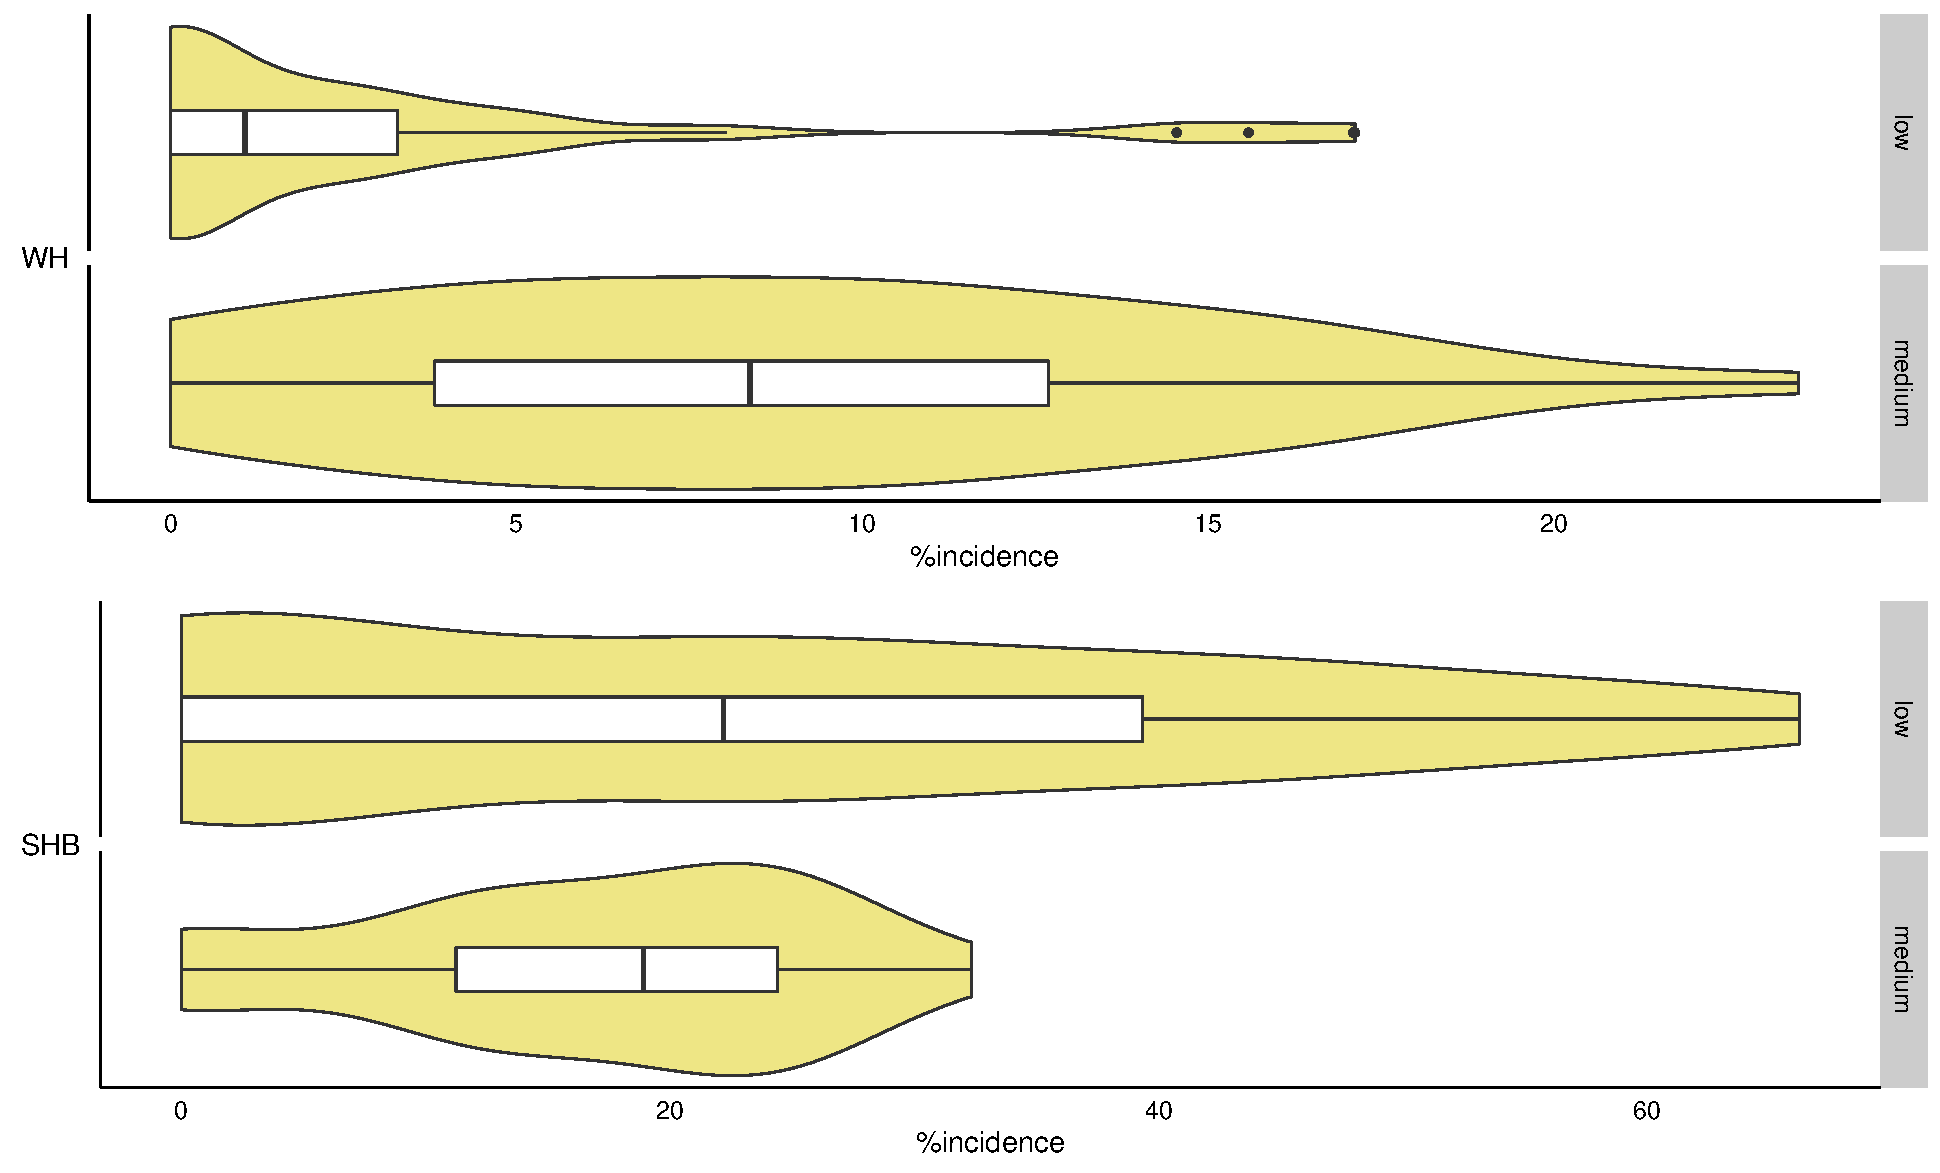
\includegraphics[width = 1\textwidth]{figures/TM_yield_box.pdf}
        \caption{.}
\label{fig:yield.box_TM}
\end{figure}

\begin{figure}
        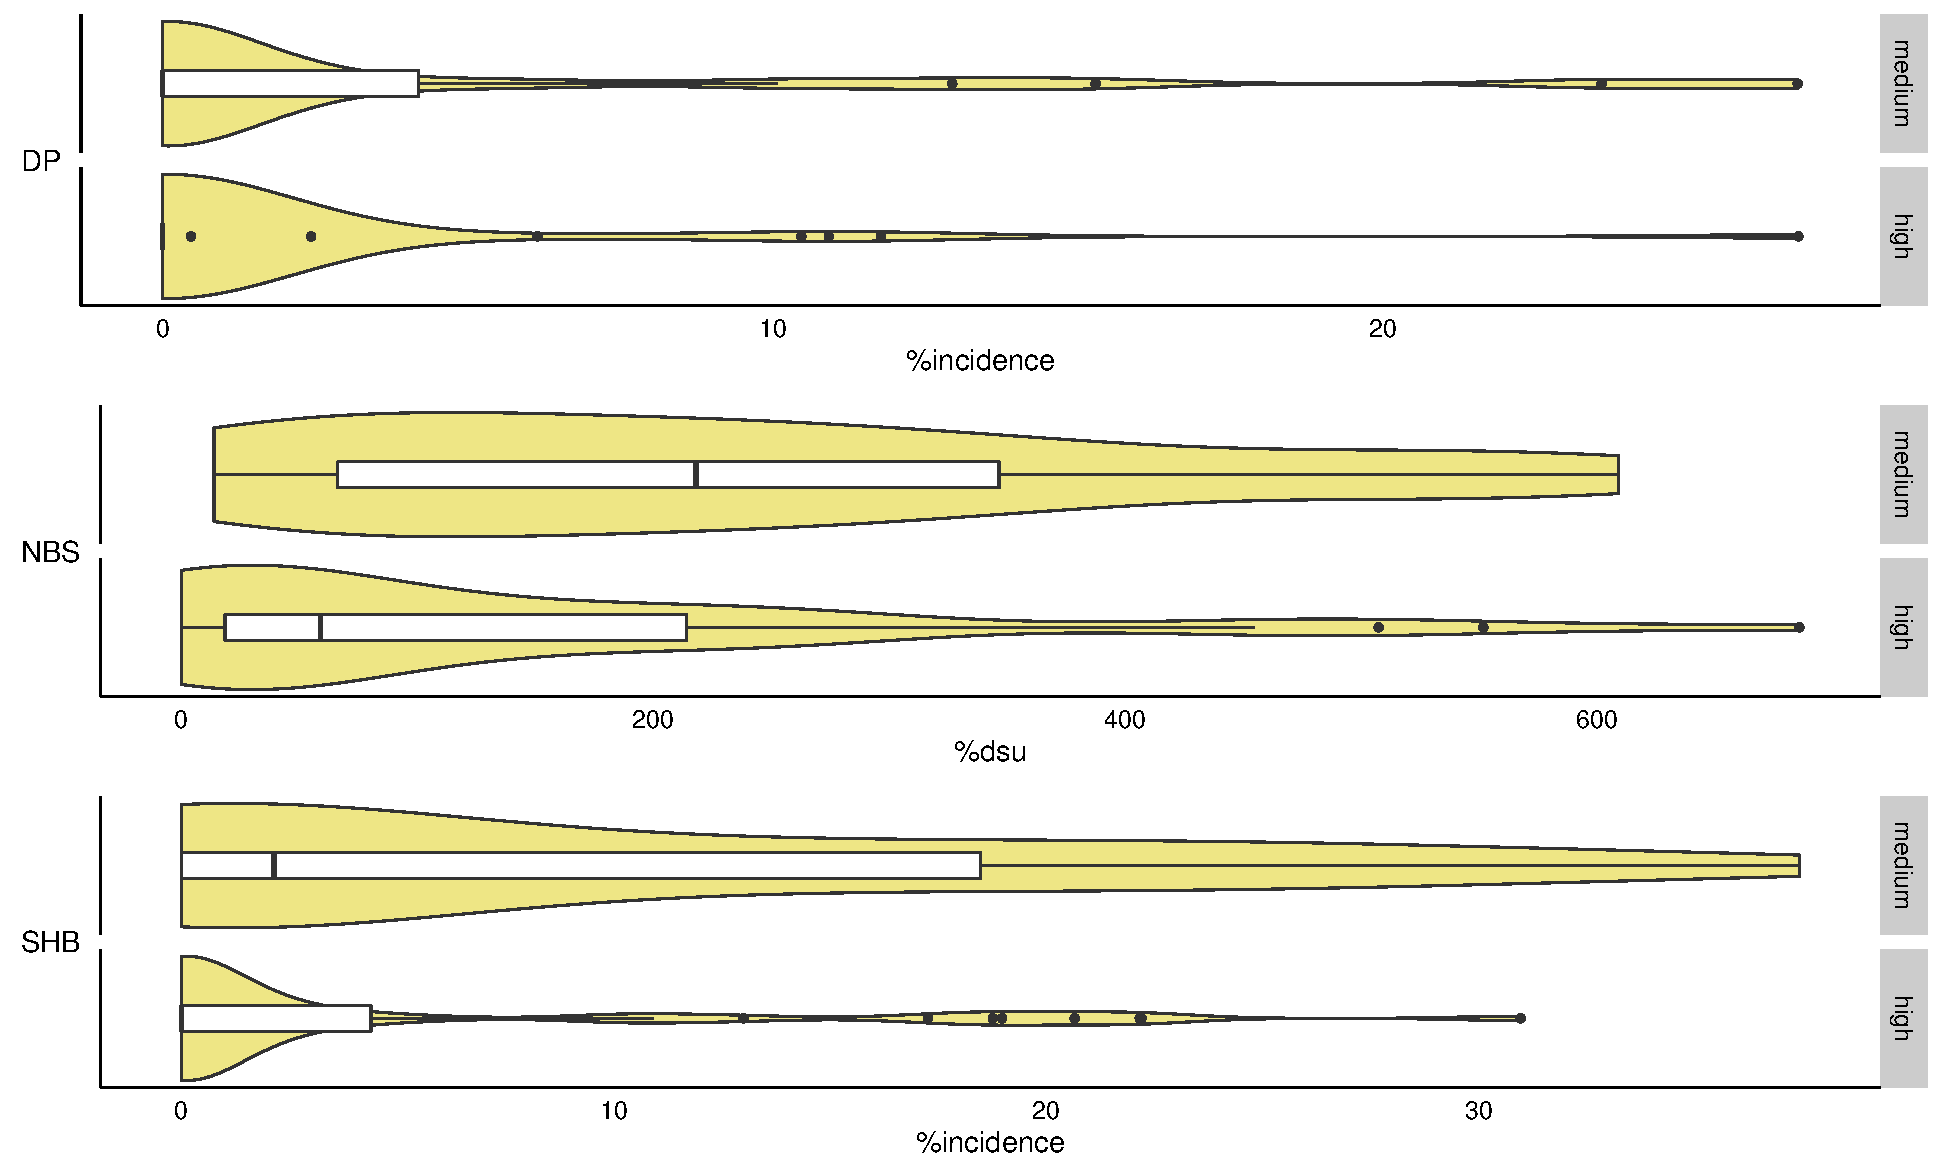
\includegraphics[width = 1\textwidth]{figures/WJ_yield_box.pdf}
        \caption{.}
\label{fig:yield.box_WJ}
\end{figure}


\clearpage
\subsection{Discussion}
When sets of changed correlations have been identified,
the next step is to establish the causal influences in the
regulatory systems (i.e. to put directions on the edges in the
undirected coexpression network) and, more importantly,
to identify which causal influences have disappeared in the
disease network with respect to the healthy network. Such
disappeared regulatory mechanisms resulted in the
observed changes in correlations and potentially could
underlie the associated disease phenotype. Although it is
not trivial to identify the causal system from the correlation
patterns, the changes in correlation hint at the
interesting regions of the network involved in disease
which could form the basis for further detailed analysis.
Systematic perturbations (e.g. experimental gene knockouts)
are needed to establish the edges’ direction. Particular
promise comes from so-called systems genetics
experiments in which genotyping and gene expression data
(and possibly metabolomics and proteomic

%Systems biology methods like this are in high demand as the differences between many conditions, be they neurodegenerative diseases, brain diseases, different kinds of cancers, different degrees of disease severity, and so forth, are very subtle and cannot be easily highlighted using the usual off-the-shelf clustering or biological pathways identification algorithms. Many studies investigate only the genes that are unique to a condition, in order to analyze how different the conditions are. However, we hypothesize that even the genes that are common between conditions (conditions can be physiological, treatment, or time) can contribute to the differences between conditions either by invoking different biological pathways or by invoking the same biological pathways to varying degrees. Our differential network analysis method is applicable to other studies where a sequence of activities or processes is being determined. For instance, in our time-dependent analysis of low dose ionizing radiation study we were able to show the active biological processes at 3, 8, and 24 hours [12]. Our approach can aid in identifying the few genes that may be the key players in the specific condition and, therefore, potential biomarkers or therapeutic targets for that condition.

 